% Chapter 14: Multivariate GARCH models
% Time Series Analysis -- Bachelor's programmes Economic Informatics and Economic Cybernetics, Bucharest University of Economic Studies
% GENERATED by latex/build_chapter14.py -- edit the generator, not this file.

\newcommand{\coursename}{Time Series Analysis}
% Preambul comun TSA -- Serii de timp / Time Series Analysis (Beamer, 16:9)
% Același design ca MFM și SFM (preluat din SFM, 5 octombrie 2026). Înainte de % Preambul comun TSA -- Serii de timp / Time Series Analysis (Beamer, 16:9)
% Același design ca MFM și SFM (preluat din SFM, 5 octombrie 2026). Înainte de % Preambul comun TSA -- Serii de timp / Time Series Analysis (Beamer, 16:9)
% Același design ca MFM și SFM (preluat din SFM, 5 octombrie 2026). Înainte de \input{../../latex/preamble} se definește
%   \newcommand{\coursename}{Time Series Analysis}      (EN)
%   \newcommand{\coursename}{Serii de timp}       (RO)  și  \def\tsalang{ro}
% Fișierele .tex se află în EN/Courses, EN/Seminars, RO/Cursuri, RO/Seminarii (două niveluri sub rădăcină).
% Deck-urile sînt generate de latex/build_chapterN.py / build_seminarN.py (vezi latex/tsa_build.py).

\documentclass[9pt, aspectratio=169, t]{beamer}
\providecommand{\coursename}{Time Series Analysis}

% Ensure content fits on slides
\setbeamersize{text margin left=8mm, text margin right=8mm}
% Smaller institute font (title page)
\setbeamerfont{institute}{size=\footnotesize}

%=============================================================================
% THEME AND STYLE CONFIGURATION
%=============================================================================
\usetheme{default}
% Using default theme for clean header/footer control

% Color Palette (matching Redispatch PDF)
\definecolor{MainBlue}{RGB}{26, 58, 110}
\definecolor{AccentBlue}{RGB}{26, 58, 110}
\definecolor{IDAred}{RGB}{205, 0, 0}
\definecolor{DarkGray}{RGB}{51, 51, 51}
\definecolor{MediumGray}{RGB}{128, 128, 128}
\definecolor{LightGray}{RGB}{248, 248, 248}
\definecolor{VeryLightGray}{RGB}{235, 235, 235}
\definecolor{KeynoteGray}{RGB}{218, 218, 218}
\definecolor{SectionGray}{RGB}{120, 120, 120}
\definecolor{FooterGray}{RGB}{100, 100, 100}
\definecolor{Crimson}{RGB}{220, 53, 69}
\definecolor{Forest}{RGB}{46, 125, 50}
\definecolor{Amber}{RGB}{181, 133, 63}
\definecolor{Orange}{RGB}{230, 126, 34}
\definecolor{Purple}{RGB}{142, 68, 173}

% Gradient background (exact Keynote 315° gradient: white to RGB 218,218,218)
\setbeamertemplate{background}{%
    \begin{tikzpicture}[remember picture, overlay]
        \shade[shading=axis, shading angle=315,
        top color=white, bottom color=KeynoteGray]
        (current page.south west) rectangle (current page.north east);
    \end{tikzpicture}%
}
% Fallback solid color for compatibility
\setbeamercolor{background canvas}{bg=}

\setbeamercolor{palette primary}{bg=MainBlue, fg=white}
\setbeamercolor{palette secondary}{bg=MainBlue!85, fg=white}
\setbeamercolor{palette tertiary}{bg=MainBlue!70, fg=white}
\setbeamercolor{structure}{fg=MainBlue}
\setbeamercolor{title}{fg=IDAred}
\setbeamercolor{frametitle}{fg=IDAred, bg=}
\setbeamercolor{block title}{bg=MainBlue, fg=white}
\setbeamercolor{block body}{bg=VeryLightGray, fg=DarkGray}
\setbeamercolor{block title alerted}{bg=Crimson, fg=white}
\setbeamercolor{block body alerted}{bg=Crimson!8, fg=DarkGray}
\setbeamercolor{block title example}{bg=Forest, fg=white}
\setbeamercolor{block body example}{bg=Forest!8, fg=DarkGray}
\setbeamercolor{item}{fg=MainBlue}

% Footer colors (override Madrid theme blue)
\setbeamercolor{author in head/foot}{fg=FooterGray, bg=}
\setbeamercolor{title in head/foot}{fg=FooterGray, bg=}
\setbeamercolor{date in head/foot}{fg=FooterGray, bg=}
\setbeamercolor{section in head/foot}{fg=FooterGray, bg=}
\setbeamercolor{subsection in head/foot}{fg=FooterGray, bg=}

% Bullet styles (apply everywhere including blocks)
\setbeamertemplate{itemize item}{\color{MainBlue}$\boxdot$}
\setbeamertemplate{itemize subitem}{\color{MainBlue}$\blacktriangleright$}
\setbeamertemplate{itemize subsubitem}{\color{MainBlue}\tiny$\bullet$}
\setbeamertemplate{itemize/enumerate body begin}{\normalsize}
\setbeamertemplate{itemize/enumerate subbody begin}{\normalsize}

% Item spacing - compact style
\setlength{\leftmargini}{10pt}       % Level 1: minimal indent
\setlength{\leftmarginii}{10pt}      % Level 2: minimal additional indent
% Compact list spacing (zero extra space before/after lists in blocks)
\makeatletter
\def\@listi{\leftmargin\leftmargini \topsep 0pt \parsep 0pt \itemsep 0pt}
\def\@listii{\leftmargin\leftmarginii \topsep 0pt \parsep 0pt \itemsep 0pt}
\makeatother

\setbeamertemplate{navigation symbols}{}

%=============================================================================
% CUSTOM HEADLINE
%=============================================================================
\setbeamertemplate{headline}{%
    \vskip10pt%
    \hbox to \paperwidth{%
        \hskip0.5cm%
        {\small\color{FooterGray}\renewcommand{\hyperlink}[2]{##2}\insertsectionhead}%
        \hfill%
        \textcolor{FooterGray}{\small\insertframenumber}%
        \hskip0.5cm%
    }%
    \vskip4pt%
    {\color{FooterGray}\hrule height 0.4pt}%
}

%=============================================================================
% CUSTOM FOOTER
%=============================================================================
\usepackage{fontawesome5}

\setbeamertemplate{footline}{%
    {\color{FooterGray}\hrule height 0.4pt}%
    \vskip4pt%
    \hbox to \paperwidth{%
        \hskip0.5cm%
        \textcolor{FooterGray}{\small\coursename}%
        \hfill%
        \raisebox{-0.1em}{%
            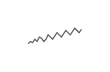
\begin{tikzpicture}[x=0.08em, y=0.08em, line width=0.4pt]
                \draw[FooterGray] (0,3) -- (1,4) -- (2,3.5) -- (3,5) -- (4,4) -- (5,6) -- (6,5.5) -- (7,4) -- (8,5) -- (9,7) -- (10,6) -- (11,5) -- (12,6.5) -- (13,8) -- (14,7) -- (15,6) -- (16,7.5) -- (17,9) -- (18,8) -- (19,7) -- (20,8.5) -- (21,10) -- (22,9) -- (23,8) -- (24,9.5);
            \end{tikzpicture}%
        }%
        \hskip0.5cm%
    }%
    \vskip6pt%
}

%=============================================================================
% PACKAGES
%=============================================================================
\usepackage[utf8]{inputenc}
\DeclareUnicodeCharacter{03B1}{\ensuremath{\alpha}}
\usepackage[T1]{fontenc}
\usepackage{amsmath, amssymb, amsthm}
\usepackage{mathtools}
\usepackage{bm}
\usepackage{tikz}
\usetikzlibrary{arrows.meta, positioning, shapes, calc, decorations.pathreplacing, shadings}
\usepackage{booktabs}
\usepackage{multirow}
\usepackage{array}
\usepackage{graphicx}
\usepackage{animate}
\usepackage{hyperref}
\usepackage{colortbl}
\usepackage{listings}
\lstset{language=Python, basicstyle=\ttfamily\scriptsize, keywordstyle=\color{MainBlue}\bfseries,
  commentstyle=\color{Forest}, stringstyle=\color{Crimson}, breaklines=true,
  frame=none, backgroundcolor=\color{VeryLightGray}, xleftmargin=2mm}
\hypersetup{colorlinks=true, linkcolor=MainBlue, urlcolor=MainBlue}
\graphicspath{{../../logos/}{../../charts/}{../../photos/}}
\usepackage{xcolor}
\hfuzz=2pt  % Suppress tiny overfull warnings (<2pt)
\vfuzz=2pt  % Suppress tiny vertical overfull warnings (<2pt)
% \mathrm in the sans-serif family of the slides (beamer resets \mathrm to the serif family at \begin{document};
% this hook runs after beamer's, so WN, Var, RMSE, ... in formulas match the surrounding text)
% Bold vectors and matrices in the same sans-serif family: \mathbf{A} in sans bold (beamer's own \mathbf came out in
% medium weight), and the bold upright Greek capitals of \boldsymbol / \bm (\bSigma, \bPhi, \boldsymbol{\Theta}) in
% cmss bold: bm.sty fixes its "boldoperators" font when it is loaded (serif cmbx), before beamer switches the
% operators to cmss, so it is reset here.
\AtBeginDocument{%
  \SetMathAlphabet{\mathrm}{normal}{\encodingdefault}{\sfdefault}{\mddefault}{n}%
  \SetMathAlphabet{\mathrm}{bold}{\encodingdefault}{\sfdefault}{bx}{n}%
  \SetMathAlphabet{\mathbf}{normal}{\encodingdefault}{\sfdefault}{bx}{n}%
  \SetMathAlphabet{\mathbf}{bold}{\encodingdefault}{\sfdefault}{bx}{n}%
  \SetSymbolFont{boldoperators}{normal}{OT1}{cmss}{bx}{n}%
  \SetSymbolFont{boldoperators}{bold}{OT1}{cmss}{bx}{n}}

%=============================================================================
% QUANTLET COMMANDS
%   \quantlet{<displayed name>}{<url>}       (generic, compatible with the older TSA decks)
%   \tsaquantlet{Ch_05}{TSA_ch5_garch}       -> https://github.com/danpele/Time-Series-Analysis/tree/main/Quantlets/Ch_05/TSA_ch5_garch
%   \qlurl{<folder>} is defined per chapter by the generator (Quantlets/Ch_NN/<folder>)
%=============================================================================
\newcommand{\tsarepo}{https://github.com/danpele/Time-Series-Analysis}
\newcommand{\tsaqlbase}{https://github.com/danpele/Time-Series-Analysis/tree/main/Quantlets}
\newcommand{\quantlet}[2]{%
    \hfill\href{#2}{%
        \raisebox{-0.15em}{
\includegraphics[height=0.7em]{ql_logo.png}}%
        \textcolor{MainBlue}{\tiny\ #1}%
    }%
}
\newcommand{\tsaquantlet}[2]{\quantlet{\detokenize{#2}}{\tsaqlbase/#1/#2}}

%=============================================================================
% NOTEBOOKS (Google Colab)
%   \colaburl{notebooks/EN/chapter5_seminar_notebook.ipynb} -> the Colab link of a file in the TSA repo
%   \nb: the chapter notebook (each seminar deck redefines it with \renewcommand)
%=============================================================================
\newcommand{\colaburl}[1]{https://colab.research.google.com/github/danpele/Time-Series-Analysis/blob/main/#1}
\newcommand{\nb}{https://colab.research.google.com/github/danpele/Time-Series-Analysis/tree/main/notebooks/EN}
\newcommand{\nbname}{notebooks/EN}

%=============================================================================
% SLIDE HELPERS (used by the generators; the same as in MFM)
%=============================================================================
% local font size for list bodies (the preamble forces \normalsize)
\newcommand{\itemsize}[1]{\setbeamertemplate{itemize/enumerate body begin}{#1}\setbeamertemplate{itemize/enumerate subbody begin}{#1}}
\newcommand{\intitle}[1]{{\hypersetup{urlcolor=white}#1}}   % white links inside coloured title bars
\newcommand{\imgcap}[1]{{\scriptsize #1}\\[0.5mm]}          % caption under a photo
\newcommand{\imgcredit}[2]{{\tiny\color{FooterGray}\href{#1}{#2}}}   % image credit: source URL, author/licence
\newcommand{\aiprompt}[1]{{\ttfamily\color{MainBlue}#1}}     % a prompt to an AI assistant

%=============================================================================
% SEMINARS: student version by default; the instructor wrapper *_solutions.tex sets \solutionstrue
%=============================================================================
\makeatletter\@ifundefined{ifsolutions}{\expandafter\newif\csname ifsolutions\endcsname}{}\makeatother
\newcommand{\solonly}[1]{\ifsolutions #1\fi}
\newcommand{\propsub}{\ifsolutions\else\framesubtitle{\ifdefined\tsalang Rezolvarea se discută la seminar\else Solution discussed in class\fi}\fi}

%=============================================================================
% APPENDIX AND CHAPTER LINKS (latex/appendix_links.py writes the calls; it also re-declares these
% macros before \begin{document}, so the decks compile with or without this preamble block)
%=============================================================================
\providecommand{\tsaapplink}[3]{\hypertarget{#2}{}\hyperlink{#1}{\beamergotobutton{#3}}}
\providecommand{\tsaappback}[2]{\begin{tikzpicture}[remember picture,overlay]\node[anchor=south east] at ([xshift=-3mm,yshift=7mm]current page.south east){\hyperlink{#1}{\beamerreturnbutton{#2}}};\end{tikzpicture}}
\providecommand{\tsachlink}[2]{\href{#1}{#2}}
\providecommand{\tsachlinkt}[2]{\href{#1}{\usebeamercolor[fg]{frametitle}#2}}

%=============================================================================
% QUANTINAR COMMAND: link către un curs Quantinar (subiecte avansate)
%=============================================================================
\newcommand{\quantinar}[2]{%
    \href{#2}{%
        \raisebox{-0.15em}{
\includegraphics[height=0.8em]{qr_logo.png}}%
        \textcolor{MainBlue}{\scriptsize\ #1}%
    }%
}

%=============================================================================
% CUSTOM TITLE PAGE
%=============================================================================
\defbeamertemplate*{title page}{hybrid}[1][]
{
    \vspace{0.2cm}
    % Logos row - top header (with clickable links)
    \begin{center}
        \href{https://www.ase.ro}{
\includegraphics[height=1.0cm]{ase_logo.png}}\hspace{0.3cm}%
        \href{https://theida.net}{
\includegraphics[height=1.0cm]{ida_logo.png}}\hspace{0.3cm}%
        \href{https://blockchain-research-center.com}{
\includegraphics[height=1.0cm]{brc_logo.png}}\hspace{0.3cm}%
        \href{https://www.ai4efin.ase.ro}{
\includegraphics[height=1.0cm]{ai4efin_logo.png}}\hspace{0.3cm}%
        \href{https://ipe.ro/new}{
\includegraphics[height=1.0cm]{acad_logo.png}}\hspace{0.3cm}%
        \href{https://www.digital-finance-msca.com}{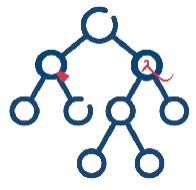
\includegraphics[height=1.0cm]{msca_logo.png}}%
    \end{center}

    \vspace{0.6cm}

    % Main title with Q logos on sides (with clickable links)
    \begin{center}
        \begin{minipage}{0.1\textwidth}
            \centering
            \href{https://quantlet.com}{
\includegraphics[height=1.1cm]{ql_logo.png}}
        \end{minipage}%
        \begin{minipage}{0.78\textwidth}
            \centering
            {\LARGE\bfseries\usebeamercolor[fg]{title}\inserttitle}

            \vspace{0.3cm}

            {\usebeamerfont{subtitle}\usebeamercolor[fg]{title}\insertsubtitle}
        \end{minipage}%
        \begin{minipage}{0.1\textwidth}
            \centering
            \href{https://quantinar.com}{
\includegraphics[height=1.1cm]{qr_logo.png}}
        \end{minipage}
    \end{center}

    \vspace{0.6cm}

    % Authors (left aligned)
    \hspace{0.5cm}{\usebeamerfont{author}\insertauthor}

    \vspace{0.3cm}

    % Institute/Affiliations (left aligned)
    \hspace{0.5cm}\begin{minipage}[t]{0.9\textwidth}
        \raggedright\small\insertinstitute
    \end{minipage}
}

%=============================================================================
% THEOREM ENVIRONMENTS
%=============================================================================
\theoremstyle{definition}
\setbeamertemplate{theorems}[numbered]
\ifdefined\tsalang
\newtheorem{defn}{Definiție}
\newtheorem{thm}{Teoremă}
\newtheorem{prop}{Propoziție}
\newtheorem{rmk}{Observație}
\else
\newtheorem{defn}{Definition}
\newtheorem{thm}{Theorem}
\newtheorem{prop}{Proposition}
\newtheorem{rmk}{Remark}
\fi

%=============================================================================
% CENTRED MINIPAGE (no extra vertical space)
%=============================================================================
\newenvironment{cminipage}[1]{%
    \par\noindent\hfill\begin{minipage}{#1}\ignorespaces
}{%
    \end{minipage}\hfill\null\par
}

%=============================================================================
% CUSTOM COMMANDS
%=============================================================================
\newcommand{\E}{\mathbb{E}}
\newcommand{\Var}{\text{Var}}
\newcommand{\Cov}{\text{Cov}}
\newcommand{\Corr}{\text{Corr}}
\newcommand{\R}{\mathbb{R}}
\newcommand{\N}{\mathbb{N}}
\newcommand{\Z}{\mathbb{Z}}
\newcommand{\B}{\mathbf{B}}
\newcommand{\imark}{\textcolor{MainBlue}{\textbullet}}
\newcommand{\RMSE}{\text{RMSE}}
\newcommand{\MAE}{\text{MAE}}
\newcommand{\MAPE}{\text{MAPE}}

% Boldface vector/matrix commands (VAR, VECM, state space; also used by the older TSA decks)
\newcommand{\bY}{\mathbf{Y}}
\newcommand{\bX}{\mathbf{X}}
\newcommand{\bA}{\mathbf{A}}
\newcommand{\bB}{\mathbf{B}}
\newcommand{\bepsilon}{\boldsymbol{\varepsilon}}
\newcommand{\bSigma}{\boldsymbol{\Sigma}}
\newcommand{\bPhi}{\boldsymbol{\Phi}}
\newcommand{\bGamma}{\boldsymbol{\Gamma}}
\newcommand{\bPi}{\boldsymbol{\Pi}}
\newcommand{\bc}{\mathbf{c}}
\newcommand{\balpha}{\boldsymbol{\alpha}}
\newcommand{\bbeta}{\boldsymbol{\beta}}
\newcommand{\bvarepsilon}{\boldsymbol{\varepsilon}}

% Legacy seminar marks (older TSA seminar decks)
\newcommand{\correct}{\textcolor{Forest}{\checkmark}}
\newcommand{\incorrect}{\textcolor{Crimson}{\texttimes}}
 se definește
%   \newcommand{\coursename}{Time Series Analysis}      (EN)
%   \newcommand{\coursename}{Serii de timp}       (RO)  și  \def\tsalang{ro}
% Fișierele .tex se află în EN/Courses, EN/Seminars, RO/Cursuri, RO/Seminarii (două niveluri sub rădăcină).
% Deck-urile sînt generate de latex/build_chapterN.py / build_seminarN.py (vezi latex/tsa_build.py).

\documentclass[9pt, aspectratio=169, t]{beamer}
\providecommand{\coursename}{Time Series Analysis}

% Ensure content fits on slides
\setbeamersize{text margin left=8mm, text margin right=8mm}
% Smaller institute font (title page)
\setbeamerfont{institute}{size=\footnotesize}

%=============================================================================
% THEME AND STYLE CONFIGURATION
%=============================================================================
\usetheme{default}
% Using default theme for clean header/footer control

% Color Palette (matching Redispatch PDF)
\definecolor{MainBlue}{RGB}{26, 58, 110}
\definecolor{AccentBlue}{RGB}{26, 58, 110}
\definecolor{IDAred}{RGB}{205, 0, 0}
\definecolor{DarkGray}{RGB}{51, 51, 51}
\definecolor{MediumGray}{RGB}{128, 128, 128}
\definecolor{LightGray}{RGB}{248, 248, 248}
\definecolor{VeryLightGray}{RGB}{235, 235, 235}
\definecolor{KeynoteGray}{RGB}{218, 218, 218}
\definecolor{SectionGray}{RGB}{120, 120, 120}
\definecolor{FooterGray}{RGB}{100, 100, 100}
\definecolor{Crimson}{RGB}{220, 53, 69}
\definecolor{Forest}{RGB}{46, 125, 50}
\definecolor{Amber}{RGB}{181, 133, 63}
\definecolor{Orange}{RGB}{230, 126, 34}
\definecolor{Purple}{RGB}{142, 68, 173}

% Gradient background (exact Keynote 315° gradient: white to RGB 218,218,218)
\setbeamertemplate{background}{%
    \begin{tikzpicture}[remember picture, overlay]
        \shade[shading=axis, shading angle=315,
        top color=white, bottom color=KeynoteGray]
        (current page.south west) rectangle (current page.north east);
    \end{tikzpicture}%
}
% Fallback solid color for compatibility
\setbeamercolor{background canvas}{bg=}

\setbeamercolor{palette primary}{bg=MainBlue, fg=white}
\setbeamercolor{palette secondary}{bg=MainBlue!85, fg=white}
\setbeamercolor{palette tertiary}{bg=MainBlue!70, fg=white}
\setbeamercolor{structure}{fg=MainBlue}
\setbeamercolor{title}{fg=IDAred}
\setbeamercolor{frametitle}{fg=IDAred, bg=}
\setbeamercolor{block title}{bg=MainBlue, fg=white}
\setbeamercolor{block body}{bg=VeryLightGray, fg=DarkGray}
\setbeamercolor{block title alerted}{bg=Crimson, fg=white}
\setbeamercolor{block body alerted}{bg=Crimson!8, fg=DarkGray}
\setbeamercolor{block title example}{bg=Forest, fg=white}
\setbeamercolor{block body example}{bg=Forest!8, fg=DarkGray}
\setbeamercolor{item}{fg=MainBlue}

% Footer colors (override Madrid theme blue)
\setbeamercolor{author in head/foot}{fg=FooterGray, bg=}
\setbeamercolor{title in head/foot}{fg=FooterGray, bg=}
\setbeamercolor{date in head/foot}{fg=FooterGray, bg=}
\setbeamercolor{section in head/foot}{fg=FooterGray, bg=}
\setbeamercolor{subsection in head/foot}{fg=FooterGray, bg=}

% Bullet styles (apply everywhere including blocks)
\setbeamertemplate{itemize item}{\color{MainBlue}$\boxdot$}
\setbeamertemplate{itemize subitem}{\color{MainBlue}$\blacktriangleright$}
\setbeamertemplate{itemize subsubitem}{\color{MainBlue}\tiny$\bullet$}
\setbeamertemplate{itemize/enumerate body begin}{\normalsize}
\setbeamertemplate{itemize/enumerate subbody begin}{\normalsize}

% Item spacing - compact style
\setlength{\leftmargini}{10pt}       % Level 1: minimal indent
\setlength{\leftmarginii}{10pt}      % Level 2: minimal additional indent
% Compact list spacing (zero extra space before/after lists in blocks)
\makeatletter
\def\@listi{\leftmargin\leftmargini \topsep 0pt \parsep 0pt \itemsep 0pt}
\def\@listii{\leftmargin\leftmarginii \topsep 0pt \parsep 0pt \itemsep 0pt}
\makeatother

\setbeamertemplate{navigation symbols}{}

%=============================================================================
% CUSTOM HEADLINE
%=============================================================================
\setbeamertemplate{headline}{%
    \vskip10pt%
    \hbox to \paperwidth{%
        \hskip0.5cm%
        {\small\color{FooterGray}\renewcommand{\hyperlink}[2]{##2}\insertsectionhead}%
        \hfill%
        \textcolor{FooterGray}{\small\insertframenumber}%
        \hskip0.5cm%
    }%
    \vskip4pt%
    {\color{FooterGray}\hrule height 0.4pt}%
}

%=============================================================================
% CUSTOM FOOTER
%=============================================================================
\usepackage{fontawesome5}

\setbeamertemplate{footline}{%
    {\color{FooterGray}\hrule height 0.4pt}%
    \vskip4pt%
    \hbox to \paperwidth{%
        \hskip0.5cm%
        \textcolor{FooterGray}{\small\coursename}%
        \hfill%
        \raisebox{-0.1em}{%
            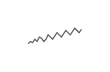
\begin{tikzpicture}[x=0.08em, y=0.08em, line width=0.4pt]
                \draw[FooterGray] (0,3) -- (1,4) -- (2,3.5) -- (3,5) -- (4,4) -- (5,6) -- (6,5.5) -- (7,4) -- (8,5) -- (9,7) -- (10,6) -- (11,5) -- (12,6.5) -- (13,8) -- (14,7) -- (15,6) -- (16,7.5) -- (17,9) -- (18,8) -- (19,7) -- (20,8.5) -- (21,10) -- (22,9) -- (23,8) -- (24,9.5);
            \end{tikzpicture}%
        }%
        \hskip0.5cm%
    }%
    \vskip6pt%
}

%=============================================================================
% PACKAGES
%=============================================================================
\usepackage[utf8]{inputenc}
\DeclareUnicodeCharacter{03B1}{\ensuremath{\alpha}}
\usepackage[T1]{fontenc}
\usepackage{amsmath, amssymb, amsthm}
\usepackage{mathtools}
\usepackage{bm}
\usepackage{tikz}
\usetikzlibrary{arrows.meta, positioning, shapes, calc, decorations.pathreplacing, shadings}
\usepackage{booktabs}
\usepackage{multirow}
\usepackage{array}
\usepackage{graphicx}
\usepackage{animate}
\usepackage{hyperref}
\usepackage{colortbl}
\usepackage{listings}
\lstset{language=Python, basicstyle=\ttfamily\scriptsize, keywordstyle=\color{MainBlue}\bfseries,
  commentstyle=\color{Forest}, stringstyle=\color{Crimson}, breaklines=true,
  frame=none, backgroundcolor=\color{VeryLightGray}, xleftmargin=2mm}
\hypersetup{colorlinks=true, linkcolor=MainBlue, urlcolor=MainBlue}
\graphicspath{{../../logos/}{../../charts/}{../../photos/}}
\usepackage{xcolor}
\hfuzz=2pt  % Suppress tiny overfull warnings (<2pt)
\vfuzz=2pt  % Suppress tiny vertical overfull warnings (<2pt)
% \mathrm in the sans-serif family of the slides (beamer resets \mathrm to the serif family at \begin{document};
% this hook runs after beamer's, so WN, Var, RMSE, ... in formulas match the surrounding text)
% Bold vectors and matrices in the same sans-serif family: \mathbf{A} in sans bold (beamer's own \mathbf came out in
% medium weight), and the bold upright Greek capitals of \boldsymbol / \bm (\bSigma, \bPhi, \boldsymbol{\Theta}) in
% cmss bold: bm.sty fixes its "boldoperators" font when it is loaded (serif cmbx), before beamer switches the
% operators to cmss, so it is reset here.
\AtBeginDocument{%
  \SetMathAlphabet{\mathrm}{normal}{\encodingdefault}{\sfdefault}{\mddefault}{n}%
  \SetMathAlphabet{\mathrm}{bold}{\encodingdefault}{\sfdefault}{bx}{n}%
  \SetMathAlphabet{\mathbf}{normal}{\encodingdefault}{\sfdefault}{bx}{n}%
  \SetMathAlphabet{\mathbf}{bold}{\encodingdefault}{\sfdefault}{bx}{n}%
  \SetSymbolFont{boldoperators}{normal}{OT1}{cmss}{bx}{n}%
  \SetSymbolFont{boldoperators}{bold}{OT1}{cmss}{bx}{n}}

%=============================================================================
% QUANTLET COMMANDS
%   \quantlet{<displayed name>}{<url>}       (generic, compatible with the older TSA decks)
%   \tsaquantlet{Ch_05}{TSA_ch5_garch}       -> https://github.com/danpele/Time-Series-Analysis/tree/main/Quantlets/Ch_05/TSA_ch5_garch
%   \qlurl{<folder>} is defined per chapter by the generator (Quantlets/Ch_NN/<folder>)
%=============================================================================
\newcommand{\tsarepo}{https://github.com/danpele/Time-Series-Analysis}
\newcommand{\tsaqlbase}{https://github.com/danpele/Time-Series-Analysis/tree/main/Quantlets}
\newcommand{\quantlet}[2]{%
    \hfill\href{#2}{%
        \raisebox{-0.15em}{
\includegraphics[height=0.7em]{ql_logo.png}}%
        \textcolor{MainBlue}{\tiny\ #1}%
    }%
}
\newcommand{\tsaquantlet}[2]{\quantlet{\detokenize{#2}}{\tsaqlbase/#1/#2}}

%=============================================================================
% NOTEBOOKS (Google Colab)
%   \colaburl{notebooks/EN/chapter5_seminar_notebook.ipynb} -> the Colab link of a file in the TSA repo
%   \nb: the chapter notebook (each seminar deck redefines it with \renewcommand)
%=============================================================================
\newcommand{\colaburl}[1]{https://colab.research.google.com/github/danpele/Time-Series-Analysis/blob/main/#1}
\newcommand{\nb}{https://colab.research.google.com/github/danpele/Time-Series-Analysis/tree/main/notebooks/EN}
\newcommand{\nbname}{notebooks/EN}

%=============================================================================
% SLIDE HELPERS (used by the generators; the same as in MFM)
%=============================================================================
% local font size for list bodies (the preamble forces \normalsize)
\newcommand{\itemsize}[1]{\setbeamertemplate{itemize/enumerate body begin}{#1}\setbeamertemplate{itemize/enumerate subbody begin}{#1}}
\newcommand{\intitle}[1]{{\hypersetup{urlcolor=white}#1}}   % white links inside coloured title bars
\newcommand{\imgcap}[1]{{\scriptsize #1}\\[0.5mm]}          % caption under a photo
\newcommand{\imgcredit}[2]{{\tiny\color{FooterGray}\href{#1}{#2}}}   % image credit: source URL, author/licence
\newcommand{\aiprompt}[1]{{\ttfamily\color{MainBlue}#1}}     % a prompt to an AI assistant

%=============================================================================
% SEMINARS: student version by default; the instructor wrapper *_solutions.tex sets \solutionstrue
%=============================================================================
\makeatletter\@ifundefined{ifsolutions}{\expandafter\newif\csname ifsolutions\endcsname}{}\makeatother
\newcommand{\solonly}[1]{\ifsolutions #1\fi}
\newcommand{\propsub}{\ifsolutions\else\framesubtitle{\ifdefined\tsalang Rezolvarea se discută la seminar\else Solution discussed in class\fi}\fi}

%=============================================================================
% APPENDIX AND CHAPTER LINKS (latex/appendix_links.py writes the calls; it also re-declares these
% macros before \begin{document}, so the decks compile with or without this preamble block)
%=============================================================================
\providecommand{\tsaapplink}[3]{\hypertarget{#2}{}\hyperlink{#1}{\beamergotobutton{#3}}}
\providecommand{\tsaappback}[2]{\begin{tikzpicture}[remember picture,overlay]\node[anchor=south east] at ([xshift=-3mm,yshift=7mm]current page.south east){\hyperlink{#1}{\beamerreturnbutton{#2}}};\end{tikzpicture}}
\providecommand{\tsachlink}[2]{\href{#1}{#2}}
\providecommand{\tsachlinkt}[2]{\href{#1}{\usebeamercolor[fg]{frametitle}#2}}

%=============================================================================
% QUANTINAR COMMAND: link către un curs Quantinar (subiecte avansate)
%=============================================================================
\newcommand{\quantinar}[2]{%
    \href{#2}{%
        \raisebox{-0.15em}{
\includegraphics[height=0.8em]{qr_logo.png}}%
        \textcolor{MainBlue}{\scriptsize\ #1}%
    }%
}

%=============================================================================
% CUSTOM TITLE PAGE
%=============================================================================
\defbeamertemplate*{title page}{hybrid}[1][]
{
    \vspace{0.2cm}
    % Logos row - top header (with clickable links)
    \begin{center}
        \href{https://www.ase.ro}{
\includegraphics[height=1.0cm]{ase_logo.png}}\hspace{0.3cm}%
        \href{https://theida.net}{
\includegraphics[height=1.0cm]{ida_logo.png}}\hspace{0.3cm}%
        \href{https://blockchain-research-center.com}{
\includegraphics[height=1.0cm]{brc_logo.png}}\hspace{0.3cm}%
        \href{https://www.ai4efin.ase.ro}{
\includegraphics[height=1.0cm]{ai4efin_logo.png}}\hspace{0.3cm}%
        \href{https://ipe.ro/new}{
\includegraphics[height=1.0cm]{acad_logo.png}}\hspace{0.3cm}%
        \href{https://www.digital-finance-msca.com}{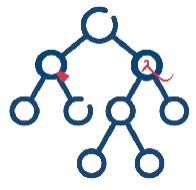
\includegraphics[height=1.0cm]{msca_logo.png}}%
    \end{center}

    \vspace{0.6cm}

    % Main title with Q logos on sides (with clickable links)
    \begin{center}
        \begin{minipage}{0.1\textwidth}
            \centering
            \href{https://quantlet.com}{
\includegraphics[height=1.1cm]{ql_logo.png}}
        \end{minipage}%
        \begin{minipage}{0.78\textwidth}
            \centering
            {\LARGE\bfseries\usebeamercolor[fg]{title}\inserttitle}

            \vspace{0.3cm}

            {\usebeamerfont{subtitle}\usebeamercolor[fg]{title}\insertsubtitle}
        \end{minipage}%
        \begin{minipage}{0.1\textwidth}
            \centering
            \href{https://quantinar.com}{
\includegraphics[height=1.1cm]{qr_logo.png}}
        \end{minipage}
    \end{center}

    \vspace{0.6cm}

    % Authors (left aligned)
    \hspace{0.5cm}{\usebeamerfont{author}\insertauthor}

    \vspace{0.3cm}

    % Institute/Affiliations (left aligned)
    \hspace{0.5cm}\begin{minipage}[t]{0.9\textwidth}
        \raggedright\small\insertinstitute
    \end{minipage}
}

%=============================================================================
% THEOREM ENVIRONMENTS
%=============================================================================
\theoremstyle{definition}
\setbeamertemplate{theorems}[numbered]
\ifdefined\tsalang
\newtheorem{defn}{Definiție}
\newtheorem{thm}{Teoremă}
\newtheorem{prop}{Propoziție}
\newtheorem{rmk}{Observație}
\else
\newtheorem{defn}{Definition}
\newtheorem{thm}{Theorem}
\newtheorem{prop}{Proposition}
\newtheorem{rmk}{Remark}
\fi

%=============================================================================
% CENTRED MINIPAGE (no extra vertical space)
%=============================================================================
\newenvironment{cminipage}[1]{%
    \par\noindent\hfill\begin{minipage}{#1}\ignorespaces
}{%
    \end{minipage}\hfill\null\par
}

%=============================================================================
% CUSTOM COMMANDS
%=============================================================================
\newcommand{\E}{\mathbb{E}}
\newcommand{\Var}{\text{Var}}
\newcommand{\Cov}{\text{Cov}}
\newcommand{\Corr}{\text{Corr}}
\newcommand{\R}{\mathbb{R}}
\newcommand{\N}{\mathbb{N}}
\newcommand{\Z}{\mathbb{Z}}
\newcommand{\B}{\mathbf{B}}
\newcommand{\imark}{\textcolor{MainBlue}{\textbullet}}
\newcommand{\RMSE}{\text{RMSE}}
\newcommand{\MAE}{\text{MAE}}
\newcommand{\MAPE}{\text{MAPE}}

% Boldface vector/matrix commands (VAR, VECM, state space; also used by the older TSA decks)
\newcommand{\bY}{\mathbf{Y}}
\newcommand{\bX}{\mathbf{X}}
\newcommand{\bA}{\mathbf{A}}
\newcommand{\bB}{\mathbf{B}}
\newcommand{\bepsilon}{\boldsymbol{\varepsilon}}
\newcommand{\bSigma}{\boldsymbol{\Sigma}}
\newcommand{\bPhi}{\boldsymbol{\Phi}}
\newcommand{\bGamma}{\boldsymbol{\Gamma}}
\newcommand{\bPi}{\boldsymbol{\Pi}}
\newcommand{\bc}{\mathbf{c}}
\newcommand{\balpha}{\boldsymbol{\alpha}}
\newcommand{\bbeta}{\boldsymbol{\beta}}
\newcommand{\bvarepsilon}{\boldsymbol{\varepsilon}}

% Legacy seminar marks (older TSA seminar decks)
\newcommand{\correct}{\textcolor{Forest}{\checkmark}}
\newcommand{\incorrect}{\textcolor{Crimson}{\texttimes}}
 se definește
%   \newcommand{\coursename}{Time Series Analysis}      (EN)
%   \newcommand{\coursename}{Serii de timp}       (RO)  și  \def\tsalang{ro}
% Fișierele .tex se află în EN/Courses, EN/Seminars, RO/Cursuri, RO/Seminarii (două niveluri sub rădăcină).
% Deck-urile sînt generate de latex/build_chapterN.py / build_seminarN.py (vezi latex/tsa_build.py).

\documentclass[9pt, aspectratio=169, t]{beamer}
\providecommand{\coursename}{Time Series Analysis}

% Ensure content fits on slides
\setbeamersize{text margin left=8mm, text margin right=8mm}
% Smaller institute font (title page)
\setbeamerfont{institute}{size=\footnotesize}

%=============================================================================
% THEME AND STYLE CONFIGURATION
%=============================================================================
\usetheme{default}
% Using default theme for clean header/footer control

% Color Palette (matching Redispatch PDF)
\definecolor{MainBlue}{RGB}{26, 58, 110}
\definecolor{AccentBlue}{RGB}{26, 58, 110}
\definecolor{IDAred}{RGB}{205, 0, 0}
\definecolor{DarkGray}{RGB}{51, 51, 51}
\definecolor{MediumGray}{RGB}{128, 128, 128}
\definecolor{LightGray}{RGB}{248, 248, 248}
\definecolor{VeryLightGray}{RGB}{235, 235, 235}
\definecolor{KeynoteGray}{RGB}{218, 218, 218}
\definecolor{SectionGray}{RGB}{120, 120, 120}
\definecolor{FooterGray}{RGB}{100, 100, 100}
\definecolor{Crimson}{RGB}{220, 53, 69}
\definecolor{Forest}{RGB}{46, 125, 50}
\definecolor{Amber}{RGB}{181, 133, 63}
\definecolor{Orange}{RGB}{230, 126, 34}
\definecolor{Purple}{RGB}{142, 68, 173}

% Gradient background (exact Keynote 315° gradient: white to RGB 218,218,218)
\setbeamertemplate{background}{%
    \begin{tikzpicture}[remember picture, overlay]
        \shade[shading=axis, shading angle=315,
        top color=white, bottom color=KeynoteGray]
        (current page.south west) rectangle (current page.north east);
    \end{tikzpicture}%
}
% Fallback solid color for compatibility
\setbeamercolor{background canvas}{bg=}

\setbeamercolor{palette primary}{bg=MainBlue, fg=white}
\setbeamercolor{palette secondary}{bg=MainBlue!85, fg=white}
\setbeamercolor{palette tertiary}{bg=MainBlue!70, fg=white}
\setbeamercolor{structure}{fg=MainBlue}
\setbeamercolor{title}{fg=IDAred}
\setbeamercolor{frametitle}{fg=IDAred, bg=}
\setbeamercolor{block title}{bg=MainBlue, fg=white}
\setbeamercolor{block body}{bg=VeryLightGray, fg=DarkGray}
\setbeamercolor{block title alerted}{bg=Crimson, fg=white}
\setbeamercolor{block body alerted}{bg=Crimson!8, fg=DarkGray}
\setbeamercolor{block title example}{bg=Forest, fg=white}
\setbeamercolor{block body example}{bg=Forest!8, fg=DarkGray}
\setbeamercolor{item}{fg=MainBlue}

% Footer colors (override Madrid theme blue)
\setbeamercolor{author in head/foot}{fg=FooterGray, bg=}
\setbeamercolor{title in head/foot}{fg=FooterGray, bg=}
\setbeamercolor{date in head/foot}{fg=FooterGray, bg=}
\setbeamercolor{section in head/foot}{fg=FooterGray, bg=}
\setbeamercolor{subsection in head/foot}{fg=FooterGray, bg=}

% Bullet styles (apply everywhere including blocks)
\setbeamertemplate{itemize item}{\color{MainBlue}$\boxdot$}
\setbeamertemplate{itemize subitem}{\color{MainBlue}$\blacktriangleright$}
\setbeamertemplate{itemize subsubitem}{\color{MainBlue}\tiny$\bullet$}
\setbeamertemplate{itemize/enumerate body begin}{\normalsize}
\setbeamertemplate{itemize/enumerate subbody begin}{\normalsize}

% Item spacing - compact style
\setlength{\leftmargini}{10pt}       % Level 1: minimal indent
\setlength{\leftmarginii}{10pt}      % Level 2: minimal additional indent
% Compact list spacing (zero extra space before/after lists in blocks)
\makeatletter
\def\@listi{\leftmargin\leftmargini \topsep 0pt \parsep 0pt \itemsep 0pt}
\def\@listii{\leftmargin\leftmarginii \topsep 0pt \parsep 0pt \itemsep 0pt}
\makeatother

\setbeamertemplate{navigation symbols}{}

%=============================================================================
% CUSTOM HEADLINE
%=============================================================================
\setbeamertemplate{headline}{%
    \vskip10pt%
    \hbox to \paperwidth{%
        \hskip0.5cm%
        {\small\color{FooterGray}\renewcommand{\hyperlink}[2]{##2}\insertsectionhead}%
        \hfill%
        \textcolor{FooterGray}{\small\insertframenumber}%
        \hskip0.5cm%
    }%
    \vskip4pt%
    {\color{FooterGray}\hrule height 0.4pt}%
}

%=============================================================================
% CUSTOM FOOTER
%=============================================================================
\usepackage{fontawesome5}

\setbeamertemplate{footline}{%
    {\color{FooterGray}\hrule height 0.4pt}%
    \vskip4pt%
    \hbox to \paperwidth{%
        \hskip0.5cm%
        \textcolor{FooterGray}{\small\coursename}%
        \hfill%
        \raisebox{-0.1em}{%
            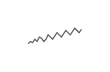
\begin{tikzpicture}[x=0.08em, y=0.08em, line width=0.4pt]
                \draw[FooterGray] (0,3) -- (1,4) -- (2,3.5) -- (3,5) -- (4,4) -- (5,6) -- (6,5.5) -- (7,4) -- (8,5) -- (9,7) -- (10,6) -- (11,5) -- (12,6.5) -- (13,8) -- (14,7) -- (15,6) -- (16,7.5) -- (17,9) -- (18,8) -- (19,7) -- (20,8.5) -- (21,10) -- (22,9) -- (23,8) -- (24,9.5);
            \end{tikzpicture}%
        }%
        \hskip0.5cm%
    }%
    \vskip6pt%
}

%=============================================================================
% PACKAGES
%=============================================================================
\usepackage[utf8]{inputenc}
\DeclareUnicodeCharacter{03B1}{\ensuremath{\alpha}}
\usepackage[T1]{fontenc}
\usepackage{amsmath, amssymb, amsthm}
\usepackage{mathtools}
\usepackage{bm}
\usepackage{tikz}
\usetikzlibrary{arrows.meta, positioning, shapes, calc, decorations.pathreplacing, shadings}
\usepackage{booktabs}
\usepackage{multirow}
\usepackage{array}
\usepackage{graphicx}
\usepackage{animate}
\usepackage{hyperref}
\usepackage{colortbl}
\usepackage{listings}
\lstset{language=Python, basicstyle=\ttfamily\scriptsize, keywordstyle=\color{MainBlue}\bfseries,
  commentstyle=\color{Forest}, stringstyle=\color{Crimson}, breaklines=true,
  frame=none, backgroundcolor=\color{VeryLightGray}, xleftmargin=2mm}
\hypersetup{colorlinks=true, linkcolor=MainBlue, urlcolor=MainBlue}
\graphicspath{{../../logos/}{../../charts/}{../../photos/}}
\usepackage{xcolor}
\hfuzz=2pt  % Suppress tiny overfull warnings (<2pt)
\vfuzz=2pt  % Suppress tiny vertical overfull warnings (<2pt)
% \mathrm in the sans-serif family of the slides (beamer resets \mathrm to the serif family at \begin{document};
% this hook runs after beamer's, so WN, Var, RMSE, ... in formulas match the surrounding text)
% Bold vectors and matrices in the same sans-serif family: \mathbf{A} in sans bold (beamer's own \mathbf came out in
% medium weight), and the bold upright Greek capitals of \boldsymbol / \bm (\bSigma, \bPhi, \boldsymbol{\Theta}) in
% cmss bold: bm.sty fixes its "boldoperators" font when it is loaded (serif cmbx), before beamer switches the
% operators to cmss, so it is reset here.
\AtBeginDocument{%
  \SetMathAlphabet{\mathrm}{normal}{\encodingdefault}{\sfdefault}{\mddefault}{n}%
  \SetMathAlphabet{\mathrm}{bold}{\encodingdefault}{\sfdefault}{bx}{n}%
  \SetMathAlphabet{\mathbf}{normal}{\encodingdefault}{\sfdefault}{bx}{n}%
  \SetMathAlphabet{\mathbf}{bold}{\encodingdefault}{\sfdefault}{bx}{n}%
  \SetSymbolFont{boldoperators}{normal}{OT1}{cmss}{bx}{n}%
  \SetSymbolFont{boldoperators}{bold}{OT1}{cmss}{bx}{n}}

%=============================================================================
% QUANTLET COMMANDS
%   \quantlet{<displayed name>}{<url>}       (generic, compatible with the older TSA decks)
%   \tsaquantlet{Ch_05}{TSA_ch5_garch}       -> https://github.com/danpele/Time-Series-Analysis/tree/main/Quantlets/Ch_05/TSA_ch5_garch
%   \qlurl{<folder>} is defined per chapter by the generator (Quantlets/Ch_NN/<folder>)
%=============================================================================
\newcommand{\tsarepo}{https://github.com/danpele/Time-Series-Analysis}
\newcommand{\tsaqlbase}{https://github.com/danpele/Time-Series-Analysis/tree/main/Quantlets}
\newcommand{\quantlet}[2]{%
    \hfill\href{#2}{%
        \raisebox{-0.15em}{
\includegraphics[height=0.7em]{ql_logo.png}}%
        \textcolor{MainBlue}{\tiny\ #1}%
    }%
}
\newcommand{\tsaquantlet}[2]{\quantlet{\detokenize{#2}}{\tsaqlbase/#1/#2}}

%=============================================================================
% NOTEBOOKS (Google Colab)
%   \colaburl{notebooks/EN/chapter5_seminar_notebook.ipynb} -> the Colab link of a file in the TSA repo
%   \nb: the chapter notebook (each seminar deck redefines it with \renewcommand)
%=============================================================================
\newcommand{\colaburl}[1]{https://colab.research.google.com/github/danpele/Time-Series-Analysis/blob/main/#1}
\newcommand{\nb}{https://colab.research.google.com/github/danpele/Time-Series-Analysis/tree/main/notebooks/EN}
\newcommand{\nbname}{notebooks/EN}

%=============================================================================
% SLIDE HELPERS (used by the generators; the same as in MFM)
%=============================================================================
% local font size for list bodies (the preamble forces \normalsize)
\newcommand{\itemsize}[1]{\setbeamertemplate{itemize/enumerate body begin}{#1}\setbeamertemplate{itemize/enumerate subbody begin}{#1}}
\newcommand{\intitle}[1]{{\hypersetup{urlcolor=white}#1}}   % white links inside coloured title bars
\newcommand{\imgcap}[1]{{\scriptsize #1}\\[0.5mm]}          % caption under a photo
\newcommand{\imgcredit}[2]{{\tiny\color{FooterGray}\href{#1}{#2}}}   % image credit: source URL, author/licence
\newcommand{\aiprompt}[1]{{\ttfamily\color{MainBlue}#1}}     % a prompt to an AI assistant

%=============================================================================
% SEMINARS: student version by default; the instructor wrapper *_solutions.tex sets \solutionstrue
%=============================================================================
\makeatletter\@ifundefined{ifsolutions}{\expandafter\newif\csname ifsolutions\endcsname}{}\makeatother
\newcommand{\solonly}[1]{\ifsolutions #1\fi}
\newcommand{\propsub}{\ifsolutions\else\framesubtitle{\ifdefined\tsalang Rezolvarea se discută la seminar\else Solution discussed in class\fi}\fi}

%=============================================================================
% APPENDIX AND CHAPTER LINKS (latex/appendix_links.py writes the calls; it also re-declares these
% macros before \begin{document}, so the decks compile with or without this preamble block)
%=============================================================================
\providecommand{\tsaapplink}[3]{\hypertarget{#2}{}\hyperlink{#1}{\beamergotobutton{#3}}}
\providecommand{\tsaappback}[2]{\begin{tikzpicture}[remember picture,overlay]\node[anchor=south east] at ([xshift=-3mm,yshift=7mm]current page.south east){\hyperlink{#1}{\beamerreturnbutton{#2}}};\end{tikzpicture}}
\providecommand{\tsachlink}[2]{\href{#1}{#2}}
\providecommand{\tsachlinkt}[2]{\href{#1}{\usebeamercolor[fg]{frametitle}#2}}

%=============================================================================
% QUANTINAR COMMAND: link către un curs Quantinar (subiecte avansate)
%=============================================================================
\newcommand{\quantinar}[2]{%
    \href{#2}{%
        \raisebox{-0.15em}{
\includegraphics[height=0.8em]{qr_logo.png}}%
        \textcolor{MainBlue}{\scriptsize\ #1}%
    }%
}

%=============================================================================
% CUSTOM TITLE PAGE
%=============================================================================
\defbeamertemplate*{title page}{hybrid}[1][]
{
    \vspace{0.2cm}
    % Logos row - top header (with clickable links)
    \begin{center}
        \href{https://www.ase.ro}{
\includegraphics[height=1.0cm]{ase_logo.png}}\hspace{0.3cm}%
        \href{https://theida.net}{
\includegraphics[height=1.0cm]{ida_logo.png}}\hspace{0.3cm}%
        \href{https://blockchain-research-center.com}{
\includegraphics[height=1.0cm]{brc_logo.png}}\hspace{0.3cm}%
        \href{https://www.ai4efin.ase.ro}{
\includegraphics[height=1.0cm]{ai4efin_logo.png}}\hspace{0.3cm}%
        \href{https://ipe.ro/new}{
\includegraphics[height=1.0cm]{acad_logo.png}}\hspace{0.3cm}%
        \href{https://www.digital-finance-msca.com}{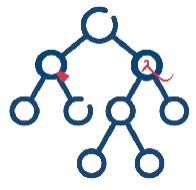
\includegraphics[height=1.0cm]{msca_logo.png}}%
    \end{center}

    \vspace{0.6cm}

    % Main title with Q logos on sides (with clickable links)
    \begin{center}
        \begin{minipage}{0.1\textwidth}
            \centering
            \href{https://quantlet.com}{
\includegraphics[height=1.1cm]{ql_logo.png}}
        \end{minipage}%
        \begin{minipage}{0.78\textwidth}
            \centering
            {\LARGE\bfseries\usebeamercolor[fg]{title}\inserttitle}

            \vspace{0.3cm}

            {\usebeamerfont{subtitle}\usebeamercolor[fg]{title}\insertsubtitle}
        \end{minipage}%
        \begin{minipage}{0.1\textwidth}
            \centering
            \href{https://quantinar.com}{
\includegraphics[height=1.1cm]{qr_logo.png}}
        \end{minipage}
    \end{center}

    \vspace{0.6cm}

    % Authors (left aligned)
    \hspace{0.5cm}{\usebeamerfont{author}\insertauthor}

    \vspace{0.3cm}

    % Institute/Affiliations (left aligned)
    \hspace{0.5cm}\begin{minipage}[t]{0.9\textwidth}
        \raggedright\small\insertinstitute
    \end{minipage}
}

%=============================================================================
% THEOREM ENVIRONMENTS
%=============================================================================
\theoremstyle{definition}
\setbeamertemplate{theorems}[numbered]
\ifdefined\tsalang
\newtheorem{defn}{Definiție}
\newtheorem{thm}{Teoremă}
\newtheorem{prop}{Propoziție}
\newtheorem{rmk}{Observație}
\else
\newtheorem{defn}{Definition}
\newtheorem{thm}{Theorem}
\newtheorem{prop}{Proposition}
\newtheorem{rmk}{Remark}
\fi

%=============================================================================
% CENTRED MINIPAGE (no extra vertical space)
%=============================================================================
\newenvironment{cminipage}[1]{%
    \par\noindent\hfill\begin{minipage}{#1}\ignorespaces
}{%
    \end{minipage}\hfill\null\par
}

%=============================================================================
% CUSTOM COMMANDS
%=============================================================================
\newcommand{\E}{\mathbb{E}}
\newcommand{\Var}{\text{Var}}
\newcommand{\Cov}{\text{Cov}}
\newcommand{\Corr}{\text{Corr}}
\newcommand{\R}{\mathbb{R}}
\newcommand{\N}{\mathbb{N}}
\newcommand{\Z}{\mathbb{Z}}
\newcommand{\B}{\mathbf{B}}
\newcommand{\imark}{\textcolor{MainBlue}{\textbullet}}
\newcommand{\RMSE}{\text{RMSE}}
\newcommand{\MAE}{\text{MAE}}
\newcommand{\MAPE}{\text{MAPE}}

% Boldface vector/matrix commands (VAR, VECM, state space; also used by the older TSA decks)
\newcommand{\bY}{\mathbf{Y}}
\newcommand{\bX}{\mathbf{X}}
\newcommand{\bA}{\mathbf{A}}
\newcommand{\bB}{\mathbf{B}}
\newcommand{\bepsilon}{\boldsymbol{\varepsilon}}
\newcommand{\bSigma}{\boldsymbol{\Sigma}}
\newcommand{\bPhi}{\boldsymbol{\Phi}}
\newcommand{\bGamma}{\boldsymbol{\Gamma}}
\newcommand{\bPi}{\boldsymbol{\Pi}}
\newcommand{\bc}{\mathbf{c}}
\newcommand{\balpha}{\boldsymbol{\alpha}}
\newcommand{\bbeta}{\boldsymbol{\beta}}
\newcommand{\bvarepsilon}{\boldsymbol{\varepsilon}}

% Legacy seminar marks (older TSA seminar decks)
\newcommand{\correct}{\textcolor{Forest}{\checkmark}}
\newcommand{\incorrect}{\textcolor{Crimson}{\texttimes}}


\newcommand{\qlurl}[1]{https://github.com/danpele/Time-Series-Analysis/tree/main/Quantlets/Ch_14/#1}

% Clickable citations (DOIs verified via Crossref)
\newcommand{\refHP}{\href{https://doi.org/10.1007/978-3-031-13584-2}{Huang and Petukhina (2022)}}
\newcommand{\refEngle}{\href{https://doi.org/10.1198/073500102288618487}{Engle (2002)}}
\newcommand{\refBoll}{\href{https://doi.org/10.2307/2109358}{Bollerslev (1990)}}
\newcommand{\refBollG}{\href{https://doi.org/10.1016/0304-4076(86)90063-1}{Bollerslev (1986)}}
\newcommand{\refEK}{\href{https://doi.org/10.1017/S0266466600009063}{Engle and Kroner (1995)}}
\newcommand{\refBEW}{\href{https://doi.org/10.1086/261527}{Bollerslev, Engle and Wooldridge (1988)}}
\newcommand{\refTse}{\href{https://doi.org/10.1016/S0304-4076(99)00080-9}{Tse (2000)}}
\newcommand{\refCES}{\href{https://doi.org/10.1093/jjfinec/nbl005}{Cappiello, Engle and Sheppard (2006)}}
\newcommand{\refAielli}{\href{https://doi.org/10.1080/07350015.2013.771027}{Aielli (2013)}}
\newcommand{\refKS}{\href{https://doi.org/10.2307/2331164}{Kroner and Sultan (1993)}}
\newcommand{\refEd}{\href{https://doi.org/10.1111/j.1540-6261.1979.tb02077.x}{Ederington (1979)}}
\newcommand{\refFR}{\href{https://doi.org/10.1111/0022-1082.00494}{Forbes and Rigobon (2002)}}
\newcommand{\refLS}{\href{https://doi.org/10.1111/0022-1082.00340}{Longin and Solnik (2001)}}
\newcommand{\refBLR}{\href{https://doi.org/10.1002/jae.842}{Bauwens, Laurent and Rombouts (2006)}}
\newcommand{\refST}{\href{https://doi.org/10.1007/978-3-540-71297-8_9}{Silvennoinen and Teräsvirta (2009)}}
\newcommand{\refKupiec}{\href{https://doi.org/10.3905/jod.1995.407942}{Kupiec (1995)}}
\newcommand{\refChr}{\href{https://doi.org/10.2307/2527341}{Christoffersen (1998)}}
\newcommand{\refMark}{\href{https://doi.org/10.1111/j.1540-6261.1952.tb01525.x}{Markowitz (1952)}}
\newcommand{\refDY}{\href{https://doi.org/10.1111/j.1468-0297.2008.02208.x}{Diebold and Yilmaz (2009)}}

\title[Time Series Analysis]{Time Series Analysis}
\subtitle{Chapter 14: Multivariate GARCH models}
\author[D.T. Pele]{Daniel Traian PELE}
\institute{Bucharest University of Economic Studies\\
IDA Institute Digital Assets\\
Blockchain Research Center\\
AI4EFin Artificial Intelligence for Energy Finance\\
Romanian Academy, Institute for Economic Forecasting\\
MSCA Digital Finance}
\date{}

%=============================================================================
\providecommand{\tsaapplink}[3]{\hypertarget{#2}{}\hyperlink{#1}{\beamergotobutton{#3}}}  % APPLINKS-MACROS
\providecommand{\tsaappback}[2]{\begin{tikzpicture}[remember picture,overlay]\node[anchor=south east] at ([xshift=-3mm,yshift=7mm]current page.south east){\hyperlink{#1}{\beamerreturnbutton{#2}}};\end{tikzpicture}}  % APPLINKS-MACROS
\providecommand{\tsachlink}[2]{\href{#1}{#2}}  % APPLINKS-MACROS
\providecommand{\tsachlinkt}[2]{\href{#1}{\usebeamercolor[fg]{frametitle}#2}}  % APPLINKS-MACROS
\begin{document}
%=============================================================================

{
\setbeamertemplate{headline}{}
\setbeamertemplate{footline}{}
\begin{frame}[noframenumbering]
    \titlepage
\end{frame}
}
% BEGIN-ACRONYMS (generat de latex/acronyms.py; nu editati manual)
\begin{frame}{Acronyms used in this material}
\setbeamertemplate{itemize/enumerate body begin}{\footnotesize}
\begin{columns}[T]
\begin{column}{0.49\textwidth}
\begin{itemize}\setlength{\itemsep}{0pt}
    \item \textbf{AI}: Artificial Intelligence
    \item \textbf{BEKK}: Baba–Engle–Kraft–Kroner (multivariate GARCH model)
    \item \textbf{BET}: Bucharest Exchange Trading (index)
    \item \textbf{BNR}: Banca Națională a României (the National Bank of Romania)
    \item \textbf{CCC}: Constant Conditional Correlation (model)
    \item \textbf{CEE}: Central and Eastern Europe
    \item \textbf{CET}: Central European Time
    \item \textbf{COVID-19}: COronaVIrus Disease 2019
    \item \textbf{DCC}: Dynamic Conditional Correlation
    \item \textbf{EODHD}: EOD Historical Data (market-data provider)
    \item \textbf{EU}: European Union
    \item \textbf{FHS}: Filtered Historical Simulation
\end{itemize}
\end{column}
\begin{column}{0.49\textwidth}
\begin{itemize}\setlength{\itemsep}{0pt}
    \item \textbf{GARCH}: Generalised AutoRegressive Conditional Heteroskedasticity
    \item \textbf{LR}: Likelihood Ratio (test)
    \item \textbf{MGARCH}: Multivariate GARCH
    \item \textbf{OLS}: Ordinary Least Squares
    \item \textbf{QML}: Quasi-Maximum Likelihood
    \item \textbf{SE}: Standard Error
    \item \textbf{US}: United States
    \item \textbf{UTC}: Coordinated Universal Time (Temps Universel Coordonné)
    \item \textbf{VAR}: Vector AutoRegression
    \item \textbf{VEC}: Vector (half-vectorised) GARCH model
    \item \textbf{VECM}: Vector Error Correction Model
\end{itemize}
\end{column}
\end{columns}
\end{frame}
% END-ACRONYMS

\begin{frame}{Why this chapter}
\itemsize{\small}
\begin{itemize}
    \item \textbf{Question}: how do the risks of several assets move \textbf{together}? \tsachlink{https://danpele.github.io/Time-Series-Analysis/EN/Courses/chapter5_conditional_volatility_garch.pdf}{Chapter 5} modelled the volatility of one series at a time
    \begin{itemize}
        \item the risk of a portfolio, a hedge or the spread of a crisis depends on \textbf{covariances and correlations}, and these change in time
    \end{itemize}
    \item \textbf{Route} of the chapter
    \begin{itemize}
        \item the conditional covariance matrix $\mathbf{H}_t$ and its conditions
        \item the VEC and BEKK models; the number of parameters
        \item CCC and DCC: volatilities and correlations estimated in two steps
        \item applications: correlations in crises, portfolio VaR 1\%, hedge ratios
    \end{itemize}
    \item \textbf{Self-study chapter}
    \begin{itemize}
        \item read the slides in order, redo the worked examples, run the notebook, then answer the self-assessment and the quiz
        \item prerequisites: \tsachlink{https://danpele.github.io/Time-Series-Analysis/EN/Courses/chapter5_conditional_volatility_garch.pdf}{Chapter 5} (GARCH), \tsachlink{https://danpele.github.io/Time-Series-Analysis/EN/Courses/chapter6_var_models_granger_causality.pdf}{Chapter 6} (VAR models), \tsachlink{https://danpele.github.io/Time-Series-Analysis/EN/Courses/chapter7_cointegration_vecm.pdf}{Chapter 7} (cointegration)
    \end{itemize}
\end{itemize}
\end{frame}

\begin{frame}{Learning outcomes}
\itemsize{\small}
\begin{itemize}
    \item Explain why portfolio risk, hedging and contagion need a model for time-varying covariances
    \item Write the VEC, BEKK, CCC and DCC models and count their parameters
    \item Compute one step of the DCC recursion by hand and interpret $a$, $b$ and $a+b$
    \item Estimate a DCC model in two steps and test it against constant correlations
    \item Compute and backtest a portfolio VaR 1\% from $\mathbf{H}_t$
    \item Compute dynamic minimum-variance hedge ratios and their hedging effectiveness
\end{itemize}
\end{frame}

\begin{frame}{Reading and tools}
\itemsize{\small}
\begin{itemize}
    \item Textbook background: \refHP\ (GARCH models); surveys: \refBLR, \refST
    \begin{itemize}
        \item the original papers: \refBEW\ (VEC), \refEK\ (BEKK), \refBoll\ (CCC), \refEngle\ (DCC)
    \end{itemize}
    \item Python Quantlets of this chapter: \href{https://github.com/danpele/Time-Series-Analysis/tree/main/Quantlets/Ch_14}{Quantlets/Ch\_14}
    \begin{itemize}
        \item step 1 (univariate GARCH) uses the \texttt{arch} package; step 2 (DCC) is written out in about 40 lines of \texttt{numpy}, because \texttt{arch} has no DCC
    \end{itemize}
    \item Lecture notebook: \href{\colaburl{notebooks/EN/chapter14_lecture_notebook.ipynb}}{open in Google Colab}
    \item Video course: \quantinar{Applied Time Series Analysis with Python}{https://quantinar.com/course/137/applied-time-series-analysis-with-python}
\end{itemize}
\end{frame}


%=============================================================================
\section{Why multivariate volatility}
%=============================================================================

\begin{frame}{Three questions that need covariances}
\itemsize{\footnotesize}
\begin{itemize}
    \item \textbf{Portfolio risk}
    \begin{itemize}
        \item the variance of a portfolio with weights $\mathbf{w}$ is $\sigma_p^2 = \mathbf{w}^\top\mathbf{H}\mathbf{w}$ \refMark
        \item $\mathbf{w}$: the vector of portfolio weights; $\mathbf{H}$: the covariance matrix of the returns; $\sigma_p^2$: the portfolio variance
        \item two assets: $\sigma_p^2 = w_1^2\sigma_1^2 + w_2^2\sigma_2^2 + 2w_1w_2\rho\,\sigma_1\sigma_2$, with volatilities $\sigma_1$, $\sigma_2$ and correlation $\rho$
        \item the correlation $\rho$ decides how much diversification helps
    \end{itemize}
    \item \textbf{Hedging}
    \begin{itemize}
        \item how many units of an asset to sell to offset the risk of another
        \item the answer is a ratio of a covariance to a variance (Section 7)
    \end{itemize}
    \item \textbf{Contagion}
    \begin{itemize}
        \item do markets move more closely together in a crisis?
        \item if correlations rise exactly when volatility rises, diversification fails when it is needed most \refLS
    \end{itemize}
    \item A univariate GARCH (\tsachlink{https://danpele.github.io/Time-Series-Analysis/EN/Courses/chapter5_conditional_volatility_garch.pdf}{Chapter 5}) gives $\sigma_{1,t}$ and $\sigma_{2,t}$; this chapter adds the time-varying $\rho_t$
\end{itemize}
\end{frame}

\begin{frame}{Worked example: correlation and portfolio risk}
\itemsize{\small}
\begin{itemize}
    \item Two assets with annual volatility 20\% each, weights 50\% and 50\%
    \item $\rho = 0.2$: $\sigma_p^2 = 0.25 \cdot 400 + 0.25 \cdot 400 + 2 \cdot 0.25 \cdot 0.2 \cdot 400 = 240$, so $\sigma_p = 15.5\%$
    \item $\rho = 0.8$: $\sigma_p^2 = 200 + 2 \cdot 0.25 \cdot 0.8 \cdot 400 = 360$, so $\sigma_p = 19.0\%$
    \item The same assets and weights: the risk of the portfolio rises by more than a fifth only because the correlation rose
    \begin{itemize}
        \item a risk model that keeps $\rho$ fixed at its calm-period value underestimates the risk in a crisis
    \end{itemize}
\end{itemize}
\end{frame}

\begin{frame}{Portfolio volatility against the correlation}
\itemsize{\footnotesize}
\begin{center}
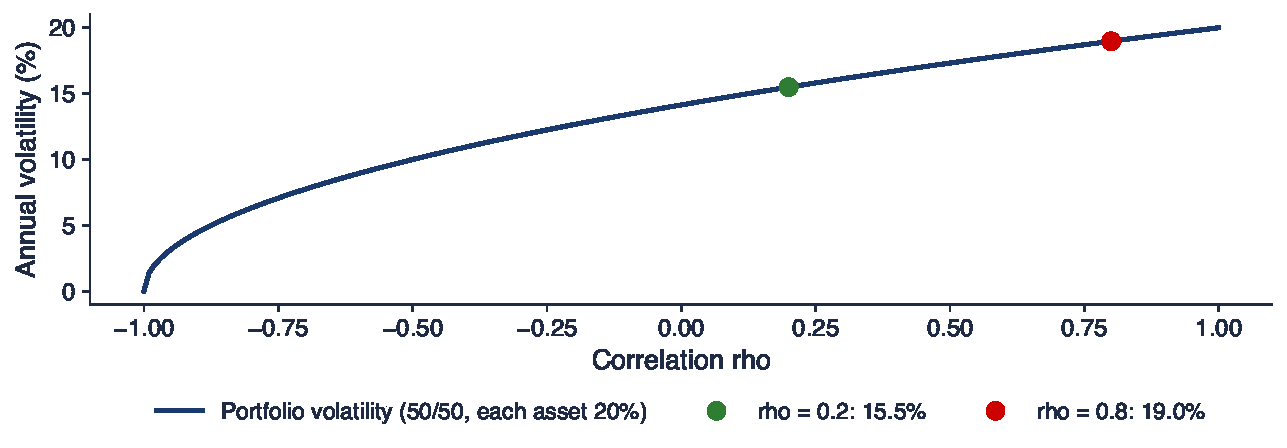
\includegraphics[width=0.97\textwidth,height=0.6\textheight,keepaspectratio]{tsa_ch14_diversification.pdf}
\end{center}
\vspace{-0.25cm}
\begin{itemize}
    \item A 50/50 portfolio of two assets with 20\% volatility each; the points are the two cases of the worked example
\end{itemize}
\quantlet{TSA\_ch14\_correlations}{\qlurl{TSA_ch14_correlations}}
\end{frame}

\begin{frame}{Interpreting the diversification curve}
\itemsize{\small}
\begin{itemize}
    \item $\rho = 1$: no diversification, $\sigma_p = 20\%$; $\rho = 0$: $\sigma_p = 20/\sqrt{2} \approx 14.1\%$; $\rho = -1$: the risk disappears
    \item The curve is concave: a rise of $\rho$ from 0.2 to 0.8 costs 15.5\% $\to$ 19.0\% of volatility
    \item The question of the chapter: does $\rho$ stay put in real markets, or does it move with the state of the market?
\end{itemize}
\end{frame}

\begin{frame}{Correlations change over time}
\itemsize{\footnotesize}
\begin{center}
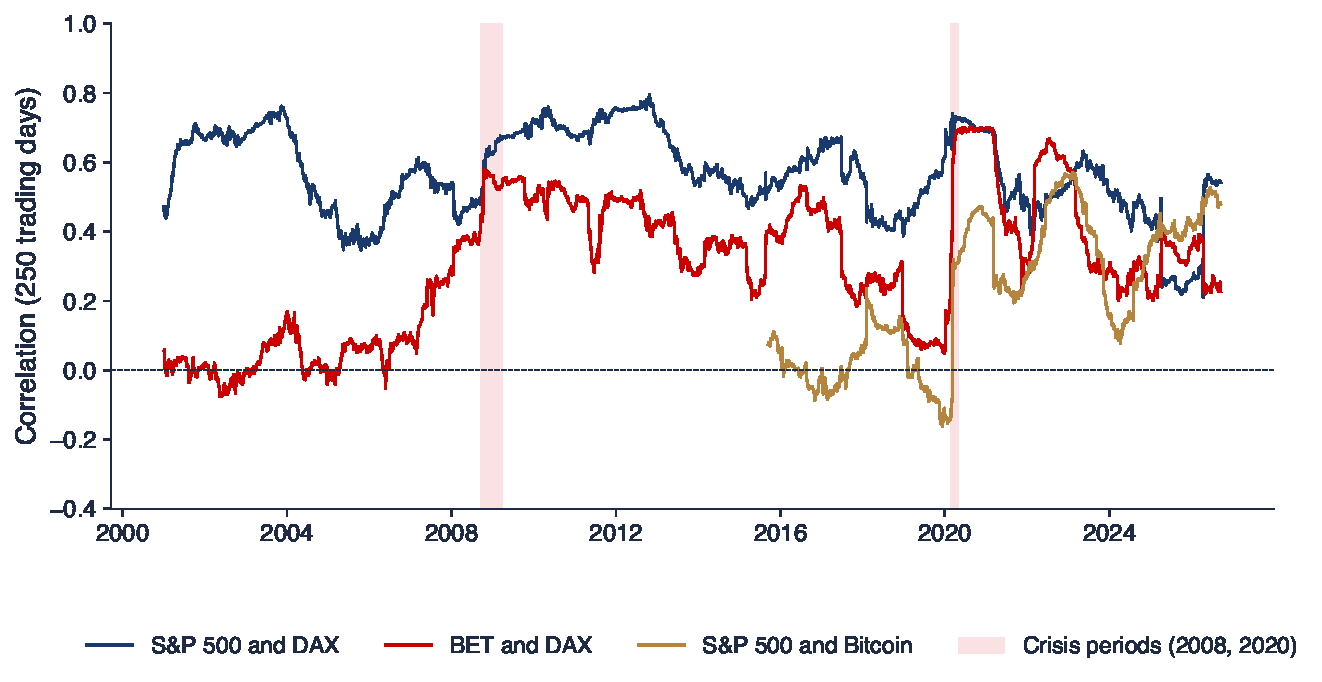
\includegraphics[width=0.97\textwidth,height=0.62\textheight,keepaspectratio]{tsa_ch14_rolling_corr.pdf}
\end{center}
\vspace{-0.25cm}
\begin{itemize}
    \item Correlation of daily log returns over rolling windows of 250 trading days (about one year), dated at the window end
    \begin{itemize}
        \item returns on the days on which both markets trade; shaded: September 2008--March 2009 and February--April 2020
    \end{itemize}
\end{itemize}
\quantlet{TSA\_ch14\_correlations}{\qlurl{TSA_ch14_correlations}}
\end{frame}

\begin{frame}{Interpreting the rolling correlations}
\itemsize{\small}
\begin{itemize}
    \item S\&P 500 and DAX: between 0.21 (April 2026) and 0.80 (October 2012); full-sample value 0.60
    \begin{itemize}
        \item the euro-area debt crisis of 2010--2012 tied the two markets even more closely than 2008
    \end{itemize}
    \item BET and DAX: close to zero before 2007 (minimum $-$0.08), up to 0.70 in August 2020: the Romanian market became integrated with Europe after EU accession
    \item S\&P 500 and Bitcoin: from $-$0.16 (December 2019) to 0.57 (February 2023); Bitcoin became a risk asset correlated with equities after 2020
    \item Correlations wander far from any constant value: a model must let them move
\end{itemize}
\end{frame}

\begin{frame}{A trap: asynchronous trading}
\itemsize{\footnotesize}
\begin{itemize}
    \item Markets close at different hours: Bucharest at 16:45 CET (17:45 local time), Frankfurt at 17:30 CET, New York at 22:00 CET; Bitcoin trades all day, every day
    \begin{itemize}
        \item news that arrives after the European close shows up in the European prices only the next day
    \end{itemize}
    \item Example: 9 April 2025, the pause of the US tariffs announced in the afternoon in New York
    \begin{itemize}
        \item 9 April: S\&P 500 +9.1\%, DAX $-$3.1\%; 10 April: S\&P 500 $-$3.5\%, DAX +4.4\%
        \item the same news, on two different days: the daily correlation is biased towards zero
    \end{itemize}
    \item Correlations of daily and weekly returns since 2015: S\&P 500 and BET 0.32 against 0.46; S\&P 500 and DAX 0.56 against 0.68; BET and DAX 0.42 against 0.47
    \begin{itemize}
        \item the gap is small for BET and DAX, which close almost together; remedies: weekly returns or returns between synchronous times
    \end{itemize}
\end{itemize}
\end{frame}

\begin{frame}{Recap: Why multivariate volatility}
\itemsize{\small}
\begin{itemize}
    \item Portfolio variance $\mathbf{w}^\top\mathbf{H}\mathbf{w}$, hedge ratios and contagion all depend on covariances
    \item Rolling correlations of real markets move a lot: integration, crises, new asset classes
    \item Check the trading hours: asynchronous closes bias daily correlations towards zero
\end{itemize}
\end{frame}


%=============================================================================
\section{The multivariate GARCH framework}
%=============================================================================

\begin{frame}{The model for $N$ return series}
\itemsize{\small}
\begin{itemize}
    \item $\mathbf{r}_t = \boldsymbol{\mu} + \boldsymbol{\varepsilon}_t$, \quad $\boldsymbol{\varepsilon}_t = \mathbf{H}_t^{1/2}\boldsymbol{\eta}_t$, \quad $\boldsymbol{\eta}_t$ i.i.d. with mean $\mathbf{0}$ and covariance $\mathbf{I}_N$
    \begin{itemize}
        \item $\mathbf{r}_t$: the vector of $N$ returns on day $t$; $\boldsymbol{\mu}$: the means (or a VAR model for the mean, \tsachlink{https://danpele.github.io/Time-Series-Analysis/EN/Courses/chapter6_var_models_granger_causality.pdf}{Chapter 6})
        \item $\mathbf{H}_t^{1/2}$: a square root of $\mathbf{H}_t$, e.g. the Cholesky factor $\mathbf{L}_t$ with $\mathbf{L}_t\mathbf{L}_t^\top = \mathbf{H}_t$
    \end{itemize}
    \item $\mathbf{H}_t = \Var(\mathbf{r}_t \mid \mathcal{F}_{t-1})$: the \textbf{conditional covariance matrix}, given the information $\mathcal{F}_{t-1}$ up to day $t-1$
    \begin{itemize}
        \item diagonal: the conditional variances $h_{ii,t} = \sigma_{i,t}^2$ (\tsachlink{https://danpele.github.io/Time-Series-Analysis/EN/Courses/chapter5_conditional_volatility_garch.pdf}{Chapter 5})
        \item off-diagonal: the conditional covariances $h_{ij,t}$; the conditional correlation is $\rho_{ij,t} = h_{ij,t}/\sqrt{h_{ii,t}h_{jj,t}}$
    \end{itemize}
    \item A \textbf{multivariate GARCH} (MGARCH) model is a rule that computes $\mathbf{H}_t$ from past shocks $\boldsymbol{\varepsilon}_{t-1}$ and past $\mathbf{H}_{t-1}$
\end{itemize}
\end{frame}

\begin{frame}{Two conditions on $\mathbf{H}_t$}
\itemsize{\small}
\begin{itemize}
    \item \textbf{Symmetry}
    \begin{itemize}
        \item $h_{ij,t} = h_{ji,t}$, so only $N(N+1)/2$ elements are distinct
        \item the operator $\mathrm{vech}$ stacks the lower triangle: $\mathrm{vech}\begin{pmatrix} h_{11} & h_{12}\\ h_{12} & h_{22}\end{pmatrix} = (h_{11}, h_{12}, h_{22})^\top$
        \item $N = 2$: 3 elements; $N = 10$: 55; $N = 50$: 1\,275
    \end{itemize}
    \item \textbf{Positive definiteness}
    \begin{itemize}
        \item $\mathbf{w}^\top\mathbf{H}_t\mathbf{w} > 0$ for every $\mathbf{w} \neq \mathbf{0}$, i.e. every portfolio has a positive variance
        \item $N = 2$: $h_{11,t} > 0$ and $h_{11,t}h_{22,t} - h_{12,t}^2 > 0$, i.e. $|\rho_{12,t}| < 1$
        \item example: $h_{11} = 4$, $h_{22} = 1$, $h_{12} = 2.5$ gives $4 - 6.25 < 0$: an impossible ``correlation'' of 1.25
    \end{itemize}
    \item A good MGARCH model guarantees both conditions for \textbf{every} $t$, with few parameters
\end{itemize}
\end{frame}

\begin{frame}{Estimation by maximum likelihood}
\itemsize{\small}
\begin{itemize}
    \item If $\boldsymbol{\eta}_t$ follows the multivariate Normal distribution, the log-likelihood is
    \begin{itemize}
        \item $\ell(\theta) = -\frac12\sum_{t=1}^{T}\left(N\log 2\pi + \log|\mathbf{H}_t| + \boldsymbol{\varepsilon}_t^\top\mathbf{H}_t^{-1}\boldsymbol{\varepsilon}_t\right)$
        \item $|\mathbf{H}_t|$ is the determinant; for $N = 1$ this is the GARCH likelihood of \tsachlink{https://danpele.github.io/Time-Series-Analysis/EN/Courses/chapter5_conditional_volatility_garch.pdf}{Chapter 5}
    \end{itemize}
    \item Returns have fat tails, so the Normal likelihood is used as \textbf{quasi-maximum likelihood} (QML)
    \begin{itemize}
        \item the estimates stay consistent; the standard errors need a robust (sandwich) correction
    \end{itemize}
    \item Every evaluation of $\ell(\theta)$ needs $\mathbf{H}_t^{-1}$ and $|\mathbf{H}_t|$ for all $t$: the cost grows fast with $N$ and with the number of parameters
\end{itemize}
\end{frame}

\begin{frame}{Recap: The multivariate GARCH framework}
\itemsize{\small}
\begin{itemize}
    \item $\mathbf{H}_t$: conditional variances on the diagonal, covariances off the diagonal; $\rho_{ij,t} = h_{ij,t}/\sqrt{h_{ii,t}h_{jj,t}}$
    \item Conditions: symmetry ($N(N+1)/2$ distinct elements) and positive definiteness
    \item Estimation by (quasi-)maximum likelihood with the multivariate Normal density
\end{itemize}
\end{frame}


%=============================================================================
\section{VEC and BEKK models}
%=============================================================================

\begin{frame}{The VEC model}
\itemsize{\footnotesize}
\begin{itemize}
    \item \refBEW: every element of $\mathbf{H}_t$ depends on every past squared shock, cross-product and element of $\mathbf{H}_{t-1}$
    \begin{itemize}
        \item VEC(1,1): $\mathrm{vech}(\mathbf{H}_t) = \mathbf{c} + \mathbf{A}\,\mathrm{vech}(\boldsymbol{\varepsilon}_{t-1}\boldsymbol{\varepsilon}_{t-1}^\top) + \mathbf{B}\,\mathrm{vech}(\mathbf{H}_{t-1})$
        \item $\boldsymbol{\varepsilon}_{t-1}\boldsymbol{\varepsilon}_{t-1}^\top$: the matrix of yesterday's squared shocks and cross-products; $\mathbf{c}$: a vector of constants; $\mathbf{A}$: the reaction to shocks; $\mathbf{B}$: the persistence
        \item with $k = N(N+1)/2$: $\mathbf{c}$ has $k$ elements, $\mathbf{A}$ and $\mathbf{B}$ are $k \times k$: in total $k + 2k^2$ parameters
    \end{itemize}
    \item $N = 2$: $k = 3$ and 21 parameters; $N = 10$: 6\,105
    \begin{itemize}
        \item and positive definiteness of $\mathbf{H}_t$ is \textbf{not} guaranteed: it needs complicated restrictions
    \end{itemize}
    \item \textbf{Diagonal VEC}
    \begin{itemize}
        \item $h_{ij,t} = c_{ij} + a_{ij}\varepsilon_{i,t-1}\varepsilon_{j,t-1} + b_{ij}h_{ij,t-1}$
        \item each element is a GARCH(1,1) of its own; $3k$ parameters (9 for $N = 2$); still no guarantee of positive definiteness
    \end{itemize}
\end{itemize}
\end{frame}

\begin{frame}{The BEKK model}
\itemsize{\footnotesize}
\begin{itemize}
    \item \refEK: $\mathbf{H}_t = \mathbf{C}\mathbf{C}^\top + \mathbf{A}^\top\boldsymbol{\varepsilon}_{t-1}\boldsymbol{\varepsilon}_{t-1}^\top\mathbf{A} + \mathbf{B}^\top\mathbf{H}_{t-1}\mathbf{B}$
    \begin{itemize}
        \item BEKK: Baba, Engle, Kraft and Kroner; $\mathbf{C}$ lower triangular, $\mathbf{A}$ and $\mathbf{B}$ are $N \times N$
        \item $\mathbf{A}$: the reaction to yesterday's shocks; $\mathbf{B}$: the persistence of $\mathbf{H}_{t-1}$; $c_{ij}^*$: the elements of $\mathbf{C}\mathbf{C}^\top$
    \end{itemize}
    \item \textbf{Positive definite by construction}
    \begin{itemize}
        \item each term is a ``square'' $\mathbf{X}^\top\mathbf{M}\mathbf{X}$ of a positive (semi)definite matrix $\mathbf{M}$
        \item $\mathbf{M}$: $\mathbf{I}$, $\boldsymbol{\varepsilon}_{t-1}\boldsymbol{\varepsilon}_{t-1}^\top$ or $\mathbf{H}_{t-1}$; $\mathbf{X}$: $\mathbf{C}^\top$, $\mathbf{A}$ or $\mathbf{B}$
        \item parameters: $N(N+1)/2 + 2N^2$, i.e. 11 for $N = 2$ and 255 for $N = 10$
    \end{itemize}
    \item \textbf{Diagonal BEKK} ($\mathbf{A}$, $\mathbf{B}$ diagonal)
    \begin{itemize}
        \item $h_{12,t} = c_{12}^* + a_{11}a_{22}\,\varepsilon_{1,t-1}\varepsilon_{2,t-1} + b_{11}b_{22}\,h_{12,t-1}$
        \item \textbf{scalar BEKK}: $\mathbf{A} = a\mathbf{I}$, $\mathbf{B} = b\mathbf{I}$, the same dynamics for all elements
    \end{itemize}
    \item The off-diagonal elements of a full $\mathbf{A}$ measure \textbf{volatility spillovers}: a shock to asset 1 raises the variance of asset 2
\end{itemize}
\end{frame}

\begin{frame}{Worked example: one step of a diagonal BEKK}
\itemsize{\small}
\begin{itemize}
    \item Given: $c_{12}^* = 0.02$, $a_{11} = 0.30$, $a_{22} = 0.25$, $b_{11} = 0.94$, $b_{22} = 0.95$, $h_{12,t-1} = 0.5$; yesterday's shocks $\varepsilon_{1,t-1} = -2$, $\varepsilon_{2,t-1} = -1.5$
    \item Step 1: the coefficients $a_{11}a_{22} = 0.075$ and $b_{11}b_{22} = 0.893$
    \item Step 2: the cross-product of shocks $\varepsilon_{1,t-1}\varepsilon_{2,t-1} = 3.000$ (both negative: a joint fall)
    \item Step 3: $h_{12,t} = 0.020 + 0.075 \cdot 3.000 + 0.893 \cdot 0.5 = 0.020 + 0.225 + 0.4465 = 0.6915$
    \item A joint fall raises the covariance from 0.5 to 0.6915; a shock of opposite signs would have lowered it
    \begin{itemize}
        \item note: a diagonal BEKK has no spillovers, because $a_{12} = a_{21} = 0$
    \end{itemize}
\end{itemize}
\end{frame}

\begin{frame}{The curse of dimensionality}
\itemsize{\footnotesize}
\begin{center}
\small
\begin{tabular}{lrrrr}
\toprule
\textbf{Model} & $N = 2$ & $N = 5$ & $N = 10$ & $N = 50$ \\
\midrule
VEC(1,1) & 21 & 465 & 6\,105 & 3\,252\,525 \\
Diagonal VEC & 9 & 45 & 165 & 3\,825 \\
BEKK(1,1) & 11 & 65 & 255 & 6\,275 \\
Diagonal BEKK & 7 & 25 & 75 & 1\,375 \\
Scalar BEKK & 5 & 17 & 57 & 1\,277 \\
CCC & 7 & 25 & 75 & 1\,375 \\
DCC & 9 & 27 & 77 & 1\,377 \\
\bottomrule
\end{tabular}
\end{center}
\begin{itemize}
    \item Number of parameters of the variance equation (the means $\boldsymbol{\mu}$ are not counted); CCC and DCC: 3 GARCH parameters per asset plus the $N(N-1)/2$ correlations, and 2 more for DCC
    \item A full VEC for 50 assets has more parameters than any sample has observations
\end{itemize}
\end{frame}

\begin{frame}{Parameters against the number of assets}
\itemsize{\footnotesize}
\begin{center}
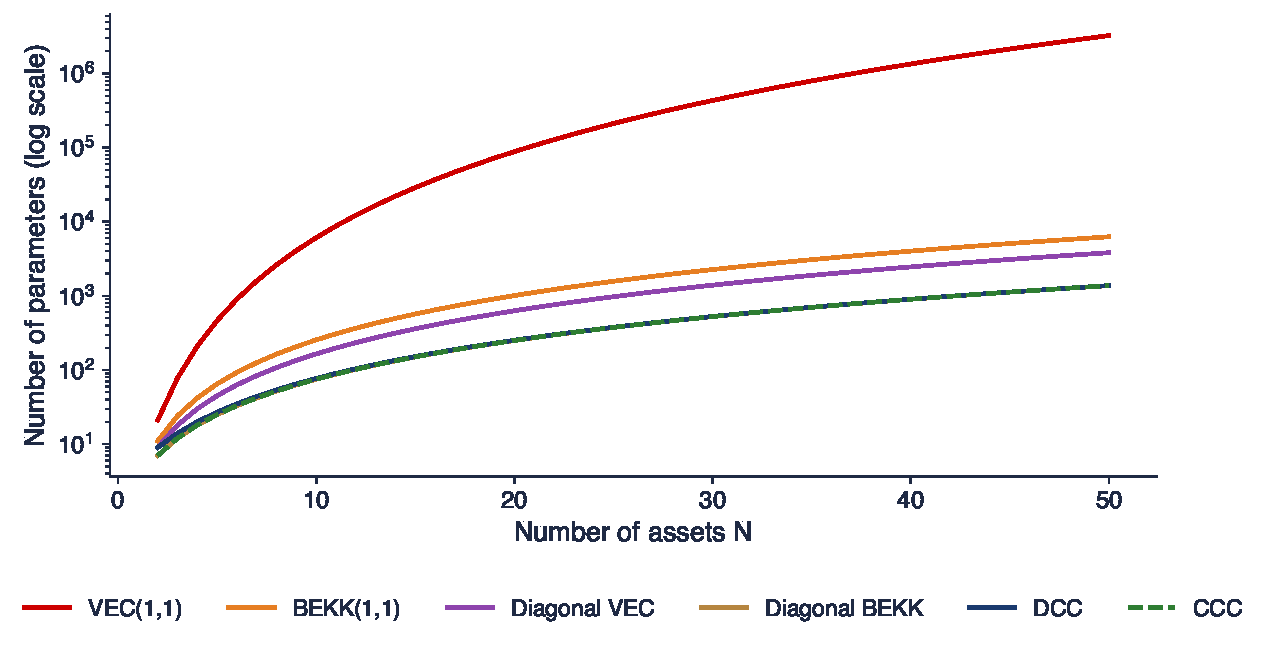
\includegraphics[width=0.97\textwidth,height=0.62\textheight,keepaspectratio]{tsa_ch14_param_count.pdf}
\end{center}
\vspace{-0.25cm}
\begin{itemize}
    \item Number of parameters of the variance equation for $N = 2, \dots, 50$ assets, log scale
\end{itemize}
\quantlet{TSA\_ch14\_parameters}{\qlurl{TSA_ch14_parameters}}
\end{frame}

\begin{frame}{Interpreting the parameter counts}
\itemsize{\small}
\begin{itemize}
    \item VEC grows like $N^4/2$, full BEKK like $2N^2$: both become impossible to estimate beyond a handful of assets
    \item CCC and DCC grow like $N^2/2$, but the correlations are \textbf{not} found by numerical optimisation: they are sample correlations (Section 4)
    \begin{itemize}
        \item the DCC optimiser works on only 2 parameters, $a$ and $b$, whatever $N$
    \end{itemize}
    \item The price of parsimony: all pairs share the same correlation dynamics
\end{itemize}
\end{frame}

\begin{frame}{Recap: VEC and BEKK}
\itemsize{\small}
\begin{itemize}
    \item VEC: the most general linear model; $k + 2k^2$ parameters, no positive-definiteness guarantee
    \item BEKK: positive definite by construction; off-diagonal $a_{ij}$ measure volatility spillovers
    \item Diagonal and scalar versions cut the parameters but remove the spillovers
\end{itemize}
\end{frame}


%=============================================================================
\section{Constant and dynamic conditional correlations}
%=============================================================================

\begin{frame}{Splitting volatilities and correlations}
\itemsize{\small}
\begin{itemize}
    \item Decomposition: $\mathbf{H}_t = \mathbf{D}_t\mathbf{R}_t\mathbf{D}_t$, \quad $\mathbf{D}_t = \mathrm{diag}(\sigma_{1,t}, \dots, \sigma_{N,t})$
    \begin{itemize}
        \item $\mathbf{R}_t$: the conditional correlation matrix (ones on the diagonal); element by element: $h_{ij,t} = \rho_{ij,t}\,\sigma_{i,t}\sigma_{j,t}$
        \item each $\sigma_{i,t}$ is a univariate GARCH(1,1) \refBollG: $\sigma_{i,t}^2 = \omega_i + \alpha_i\varepsilon_{i,t-1}^2 + \beta_i\sigma_{i,t-1}^2$
    \end{itemize}
    \item \textbf{Standardised residuals}
    \begin{itemize}
        \item $z_{i,t} = \varepsilon_{i,t}/\sigma_{i,t}$
        \item their conditional covariance matrix is exactly $\mathbf{R}_t$
    \end{itemize}
    \item \textbf{CCC} (constant conditional correlation, \refBoll)
    \begin{itemize}
        \item $\mathbf{R}_t = \mathbf{R}$ for all $t$
        \item $\mathbf{H}_t$ is positive definite whenever $\mathbf{R}$ is; $\mathbf{R}$ is estimated by the sample correlation of the $z_{i,t}$
        \item covariances still move, but only through the volatilities; the rolling correlations of Section 1 reject this
    \end{itemize}
\end{itemize}
\end{frame}

\begin{frame}{Robert Engle and the DCC model}
\itemsize{\footnotesize}
\begin{columns}[T]
\begin{column}{0.33\textwidth}
\centering

\includegraphics[height=0.42\textheight]{ch5_robert_engle_2022.jpg}\\[1mm]
\imgcap{Robert F. Engle (b.\ 1942), Nobel Prize 2003}
\imgcredit{https://commons.wikimedia.org/wiki/File:0603-Kraneshares_KRBN-RobertEngle-JonDemske-16_(cropped).jpg}{Photo: Jon Demske (2022); CC BY-SA 4.0; Wikimedia Commons}
\end{column}
\begin{column}{0.65\textwidth}
\begin{itemize}
    \item \refEngle: let the correlations follow a GARCH-like recursion
    \begin{itemize}
        \item $\mathbf{Q}_t = (1 - a - b)\,\bar{\mathbf{Q}} + a\,\mathbf{z}_{t-1}\mathbf{z}_{t-1}^\top + b\,\mathbf{Q}_{t-1}$
        \item $\mathbf{Q}_t$: an auxiliary matrix with elements $q_{ij,t}$; $\mathbf{z}_{t-1}$: yesterday's vector of standardised residuals
        \item $\rho_{ij,t} = q_{ij,t}/\sqrt{q_{ii,t}\,q_{jj,t}}$: the rescaling puts ones on the diagonal
    \end{itemize}
    \item $\bar{\mathbf{Q}}$: the unconditional correlation of $\mathbf{z}_t$, set to its sample value (\textbf{correlation targeting})
    \begin{itemize}
        \item $a \ge 0$: reaction to yesterday's joint shock; $b \ge 0$: persistence; $a + b < 1$: mean reversion to $\bar{\mathbf{Q}}$
    \end{itemize}
    \item $a = b = 0$ gives back CCC
\end{itemize}
\end{column}
\end{columns}
\end{frame}

\begin{frame}{Two-step estimation}
\itemsize{\footnotesize}
\begin{itemize}
    \item The log-likelihood splits into a volatility part and a correlation part: $\ell = \ell_V(\theta_1) + \ell_C(\theta_1, a, b)$
    \begin{itemize}
        \item $\theta_1$: the GARCH parameters of all series; $\ell_V$ depends only on them, $\ell_C$ also on $a$ and $b$
    \end{itemize}
    \item \textbf{Step 1}
    \begin{itemize}
        \item fit a GARCH(1,1) to each series separately (\tsachlink{https://danpele.github.io/Time-Series-Analysis/EN/Courses/chapter5_conditional_volatility_garch.pdf}{Chapter 5})
        \item keep $\hat\sigma_{i,t}$ and $\hat z_{i,t} = \hat\varepsilon_{i,t}/\hat\sigma_{i,t}$
    \end{itemize}
    \item \textbf{Step 2}
    \begin{itemize}
        \item set $\bar{\mathbf{Q}}$ to the sample correlation of $\hat{\mathbf{z}}_t$ and maximise over $(a, b)$ only
        \item $\ell_C(a, b) = -\frac12\sum_t\left(\log|\mathbf{R}_t| + \hat{\mathbf{z}}_t^\top\mathbf{R}_t^{-1}\hat{\mathbf{z}}_t - \hat{\mathbf{z}}_t^\top\hat{\mathbf{z}}_t\right)$
    \end{itemize}
    \item Consistent, fast, works for large $N$; the step-2 standard errors ignore the estimation error of step 1 (they are too small)
    \item \textbf{Test against CCC}
    \begin{itemize}
        \item likelihood ratio $LR = 2(\ell_C^{DCC} - \ell_C^{CCC})$, compared with $\chi^2(2)$ (5\% critical value 5.99)
        \item also \refTse
        \item $\ell_C^{DCC}$, $\ell_C^{CCC}$: the maximised correlation log-likelihoods of the two models; a large $LR$ rejects constant correlation
        \item $a = b = 0$ lies on the boundary of the parameter space, so the $\chi^2(2)$ critical value is conservative
    \end{itemize}
\end{itemize}
\end{frame}

\begin{frame}{Worked example: one step of the DCC recursion}
\itemsize{\footnotesize}
\begin{itemize}
    \item Given: $a = 0.05$, $b = 0.93$, $\bar q_{12} = 0.5$ (and $\bar q_{11} = \bar q_{22} = 1$), $\mathbf{Q}_{t-1} = \begin{pmatrix}1 & 0.5\\ 0.5 & 1\end{pmatrix}$, yesterday $z_{1,t-1} = -2$, $z_{2,t-1} = -2.5$
    \item Step 1: $1 - a - b = 0.020$
    \item Step 2: $q_{12,t} = 0.020 \cdot 0.5 + 0.05 \cdot (-2)(-2.5) + 0.93 \cdot 0.5 = 0.010 + 0.250 + 0.465 = 0.725$
    \item Step 3: $q_{11,t} = 0.020 + 0.05 \cdot 4 + 0.93 = 1.150$; \quad $q_{22,t} = 0.020 + 0.05 \cdot 6.25 + 0.93 = 1.2625$
    \item Step 4: $\rho_{12,t} = 0.725/\sqrt{1.150 \cdot 1.2625} = 0.602$
    \begin{itemize}
        \item a large joint fall raises tomorrow's correlation from 0.50 to 0.602; without step 3 the ``correlation'' $q_{12,t}$ would be 0.725
    \end{itemize}
\end{itemize}
\end{frame}

\begin{frame}{Reading $a$ and $b$}
\itemsize{\small}
\begin{itemize}
    \item $a$ is the \textbf{news} coefficient
    \begin{itemize}
        \item how much one day's joint shock moves the correlation
        \item typical daily values 0.01--0.05
    \end{itemize}
    \item $a + b$ is the \textbf{persistence}
    \begin{itemize}
        \item a deviation of $q_{ij,t}$ from $\bar q_{ij}$ shrinks by the factor $a + b$ each day
        \item half-life: $\ln 0.5/\ln(a + b)$ days; $a + b = 0.98$ gives 34 days, $0.99$ gives 69 days
    \end{itemize}
    \item The same reading as $\alpha$ and $\alpha + \beta$ in a GARCH(1,1) (\tsachlink{https://danpele.github.io/Time-Series-Analysis/EN/Courses/chapter5_conditional_volatility_garch.pdf}{Chapter 5})
    \item Variants: asymmetric DCC (joint falls move correlations more than joint rises) \refCES; corrected DCC \refAielli
\end{itemize}
\end{frame}

\begin{frame}{Recap: CCC and DCC}
\itemsize{\small}
\begin{itemize}
    \item $\mathbf{H}_t = \mathbf{D}_t\mathbf{R}_t\mathbf{D}_t$: GARCH volatilities times a correlation matrix
    \item CCC: $\mathbf{R}$ constant; DCC: $\mathbf{Q}_t$ follows a GARCH-like recursion with parameters $a$, $b$
    \item Two steps: univariate GARCH, then $(a, b)$ with correlation targeting; LR test against CCC
\end{itemize}
\end{frame}


%=============================================================================
\section{DCC for the S\&P 500 and the DAX}
%=============================================================================

\begin{frame}{Step 1: two univariate GARCH models}
\itemsize{\footnotesize}
\begin{center}
\small
\begin{tabular}{lrrrrrrr}
\toprule
\textbf{Index} & $\mu$ & $\omega$ & $\alpha$ & $\beta$ & $\alpha + \beta$ & kurt.\ $r_t$ & kurt.\ $z_t$ \\
\midrule
S\&P 500 & 0.063 & 0.027 & 0.122 & 0.857 & 0.980 & 10.5 & 1.8 \\
DAX & 0.067 & 0.030 & 0.098 & 0.886 & 0.984 & 6.2 & 1.4 \\
\bottomrule
\end{tabular}
\end{center}
\begin{itemize}
    \item Daily log returns in \%, 6\,605 common trading days, 4 January 2000--18 September 2026 (EODHD); GARCH(1,1) with a constant mean, Gaussian QML; kurt.: excess kurtosis
    \item Standardising by $\hat\sigma_{i,t}$ removes most of the excess kurtosis, but not all: the tails of $z_t$ are still fatter than Normal
    \item Correlation of the returns 0.599; correlation of the residuals $\bar q_{12} = 0.575$, the CCC estimate
\end{itemize}
\end{frame}

\begin{frame}{Step 1: conditional volatilities}
\itemsize{\footnotesize}
\begin{center}
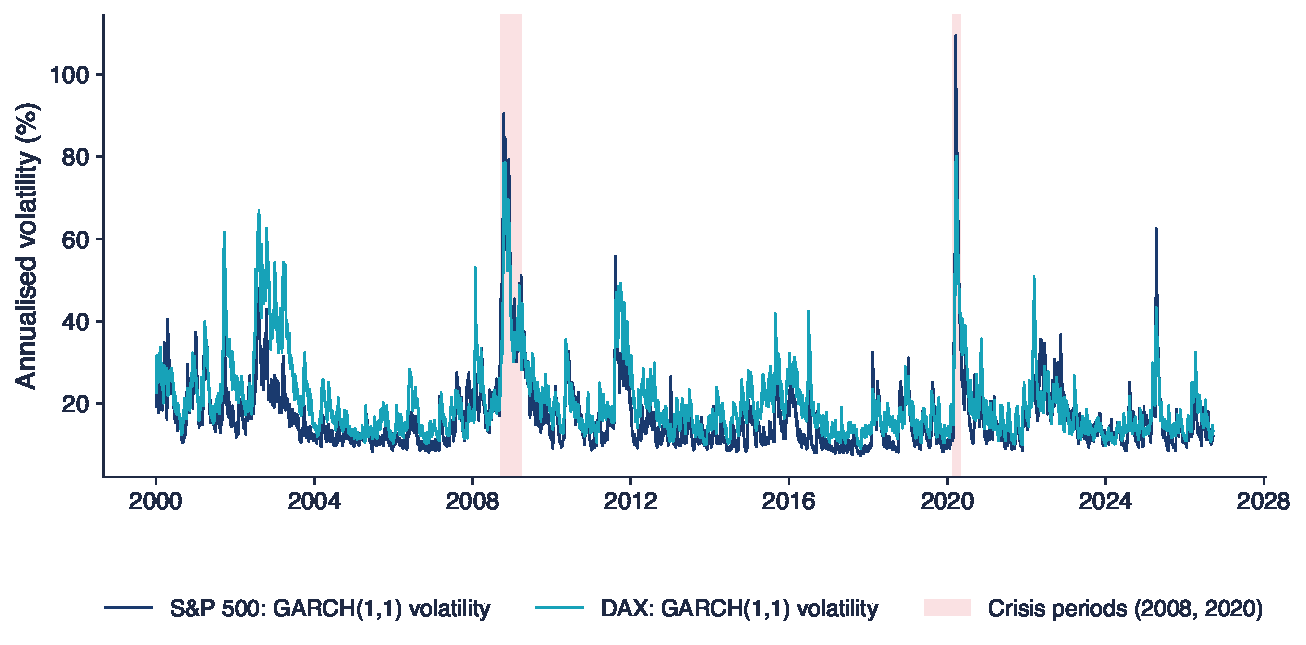
\includegraphics[width=0.97\textwidth,height=0.62\textheight,keepaspectratio]{tsa_ch14_garch_step1.pdf}
\end{center}
\vspace{-0.25cm}
\begin{itemize}
    \item One-step-ahead GARCH(1,1) volatility $\hat\sigma_{i,t}\sqrt{252}$, annualised, in \%; shaded: the crises of 2008 and 2020
\end{itemize}
\quantlet{TSA\_ch14\_dcc\_estimation}{\qlurl{TSA_ch14_dcc_estimation}}
\end{frame}

\begin{frame}{Interpreting the volatilities}
\itemsize{\small}
\begin{itemize}
    \item Both volatilities peak in the same weeks: S\&P 500 109\% on 17 March 2020, DAX 80\% on 25 March 2020
    \begin{itemize}
        \item volatility clustering happens \textbf{jointly}: the covariance rises even with a constant correlation
    \end{itemize}
    \item Persistence 0.980 and 0.984: volatility shocks fade slowly, as in \tsachlink{https://danpele.github.io/Time-Series-Analysis/EN/Courses/chapter5_conditional_volatility_garch.pdf}{Chapter 5}
    \item Step 2 asks a different question: once the volatilities are removed, is the remaining correlation constant?
\end{itemize}
\end{frame}

\begin{frame}{Step 2: the estimated DCC}
\itemsize{\footnotesize}
\begin{center}
\small
\begin{tabular}{lrr}
\toprule
\textbf{Quantity} & \textbf{Estimate} & \textbf{SE} \\
\midrule
$a$ & 0.0152 & 0.0035 \\
$b$ & 0.9766 & 0.0065 \\
$a + b$ & 0.9918 &  \\
Half-life of a correlation shock (days) & 85 &  \\
LR against CCC & 131.8 &  \\
$\chi^2(2)$ critical value, 5\% & 5.99 &  \\
\bottomrule
\end{tabular}
\end{center}
\begin{itemize}
    \item $a$ is small but well determined; $a + b$ is close to 1: correlation shocks last for months
    \item LR = 131.8 is far above 5.99: constant correlation is rejected
    \item SE: standard errors from the step-2 Hessian (too small, they ignore step 1)
\end{itemize}
\end{frame}

\begin{frame}{DCC correlation of the S\&P 500 and the DAX}
\itemsize{\footnotesize}
\begin{center}
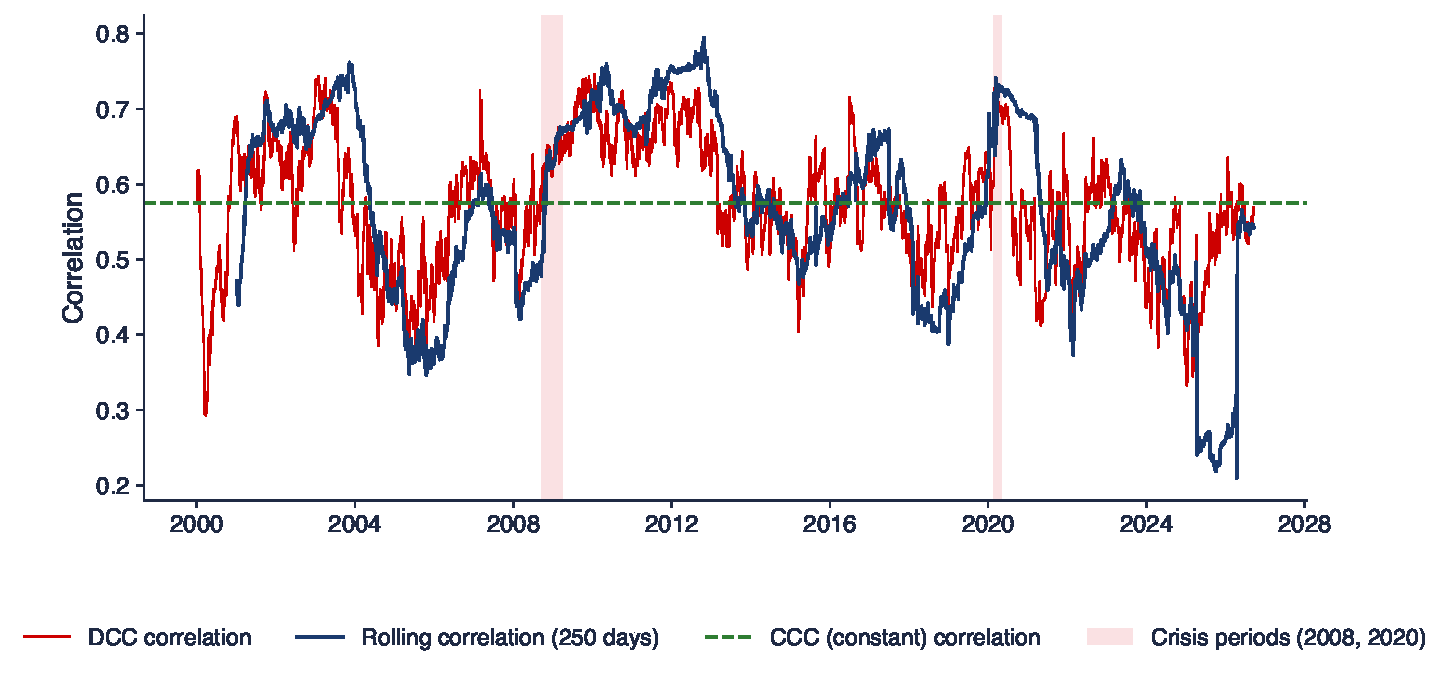
\includegraphics[width=0.97\textwidth,height=0.62\textheight,keepaspectratio]{tsa_ch14_dcc_sp_dax.pdf}
\end{center}
\vspace{-0.25cm}
\begin{itemize}
    \item One-step-ahead DCC correlation $\hat\rho_{12,t}$, the 250-day rolling correlation and the CCC value $\bar q_{12}$; daily, 4 January 2000--18 September 2026
\end{itemize}
\quantlet{TSA\_ch14\_dcc\_estimation}{\qlurl{TSA_ch14_dcc_estimation}}
\end{frame}

\begin{frame}{Interpreting the DCC correlation}
\itemsize{\small}
\begin{itemize}
    \item The DCC correlation ranges from 0.29 (March 2000) to 0.75 (January 2010), around a mean of 0.57
    \item It follows the rolling correlation, but reacts within days instead of a year and has no window to choose
    \begin{itemize}
        \item the rolling estimate is more erratic (standard deviation 0.122 against 0.083) and jumps when an extreme day enters or leaves the window
    \end{itemize}
    \item The rolling estimate falls sharply in 2025--2026: the asynchronous days of April 2025 (Section 1) pull it down for exactly 250 days
\end{itemize}
\end{frame}

\begin{frame}{Correlations in crises}
\itemsize{\footnotesize}
\begin{columns}[T]
\begin{column}{0.36\textwidth}
\centering
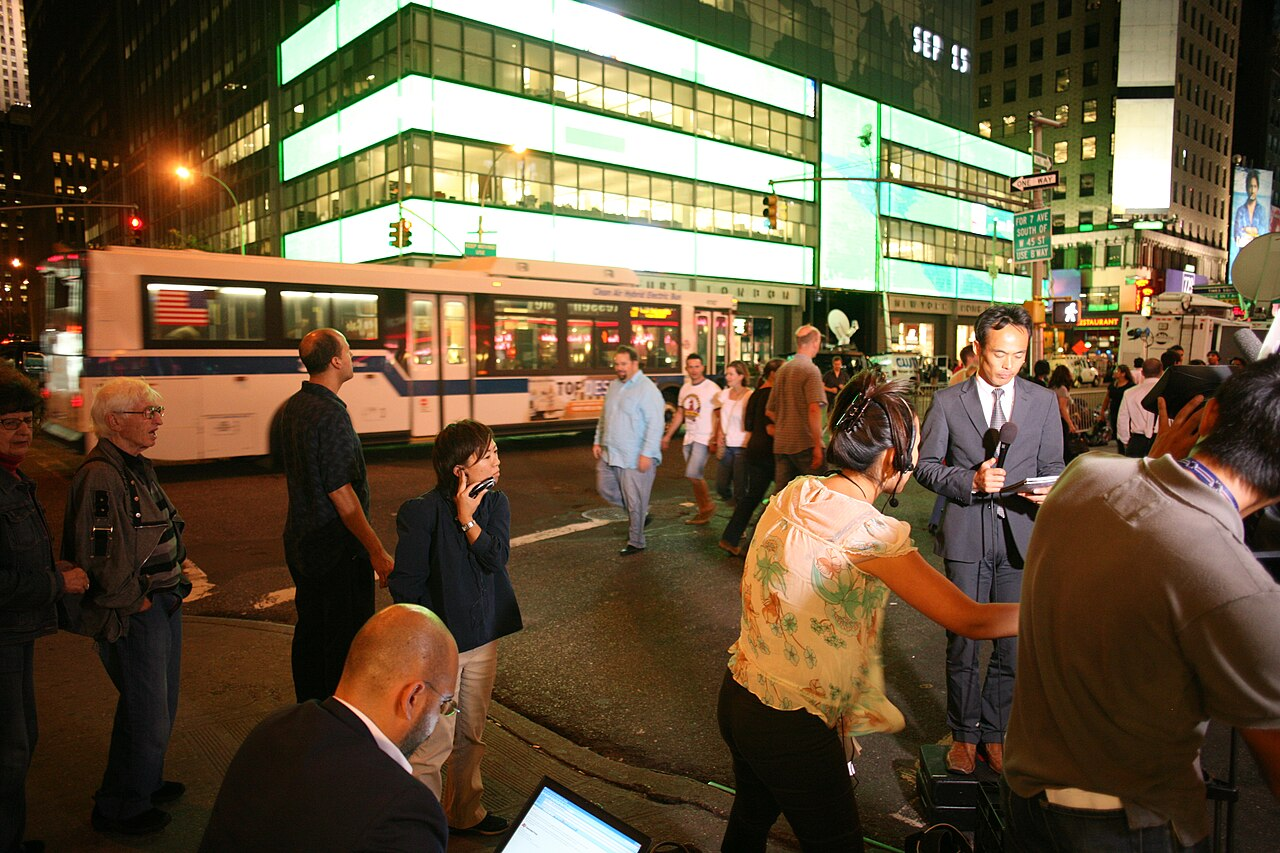
\includegraphics[height=0.36\textheight]{ch5_lehman_2008.jpg}\\[1mm]
\imgcap{Lehman Brothers, New York, 15 September 2008}
\imgcredit{https://commons.wikimedia.org/wiki/File:Lehman_Brothers-NYC-20080915.jpg}{Photo: Robert Scoble (2008); CC BY 2.0; Wikimedia Commons}
\end{column}
\begin{column}{0.62\textwidth}
\begin{center}
\footnotesize
\begin{tabular}{lrr}
\toprule
\textbf{Period} & $\bar\rho^{DCC}$ & $\bar\sigma^{S\&P}$ (\%) \\
\midrule
Calm, 2017--2019 & 0.56 & 13 \\
Sept 2008--March 2009 & 0.63 & 51 \\
Feb--April 2020 & 0.70 & 58 \\
\bottomrule
\end{tabular}
\end{center}
\begin{itemize}
    \item Average DCC correlation and average annualised S\&P 500 volatility in each period
    \item Correlations are higher in crises, but volatility rises far more
    \item Caution \refFR: the sample correlation rises mechanically when volatility rises, even if the link is unchanged; DCC reduces this effect because it works with $z_t$, not with $r_t$
\end{itemize}
\end{column}
\end{columns}
\end{frame}

\begin{frame}{Inside the crises of 2008 and 2020}
\itemsize{\footnotesize}
\begin{center}
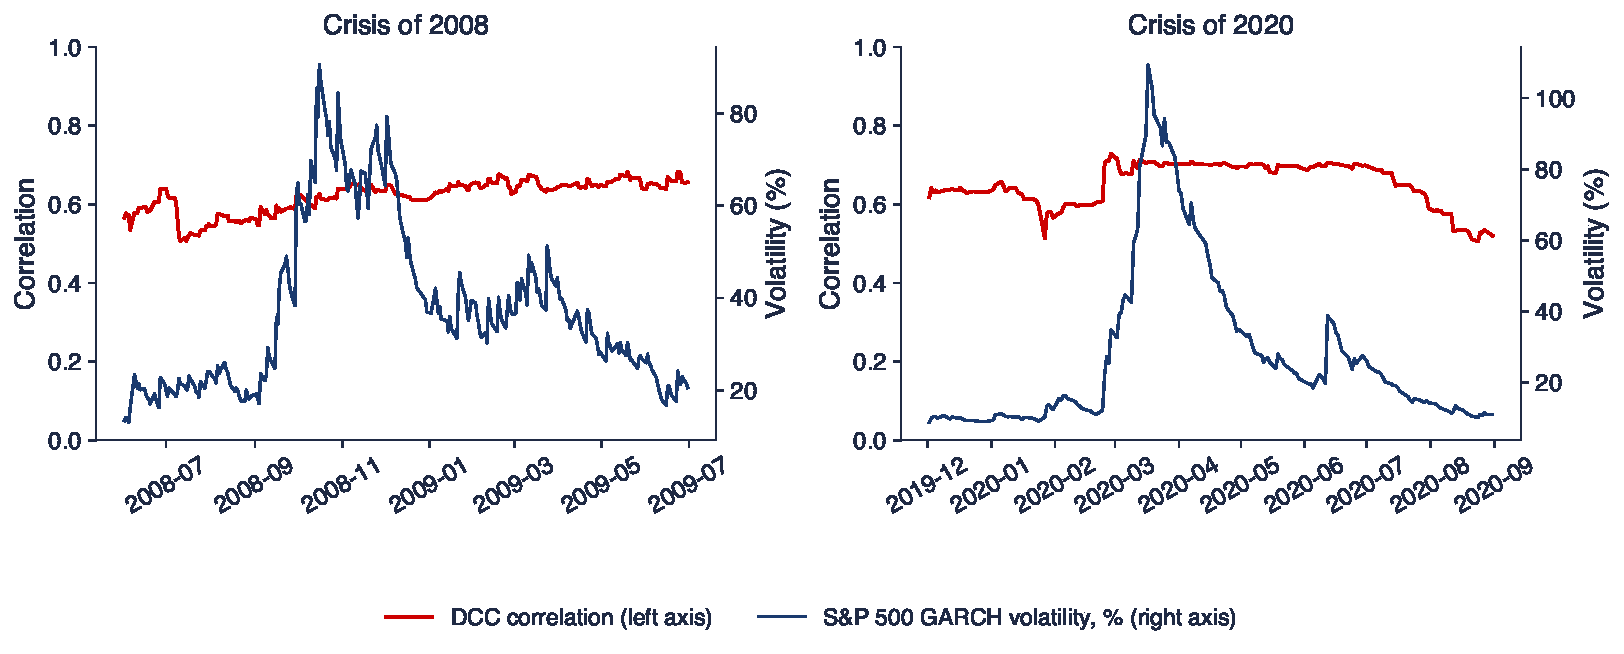
\includegraphics[width=0.97\textwidth,height=0.6\textheight,keepaspectratio]{tsa_ch14_crisis_zoom.pdf}
\end{center}
\vspace{-0.25cm}
\begin{itemize}
    \item DCC correlation of the S\&P 500 and the DAX (left axis) and the GARCH volatility of the S\&P 500 (right axis)
\end{itemize}
\quantlet{TSA\_ch14\_dcc\_estimation}{\qlurl{TSA_ch14_dcc_estimation}}
\end{frame}

\begin{frame}{Interpreting the two crises}
\itemsize{\small}
\begin{itemize}
    \item 2008: volatility peaks at 90\% on 16 October 2008, while the correlation drifts up from 0.57 to 0.68 only by 23 June 2009
    \item 2020: the correlation jumps to 0.73 on 28 February 2020, before the volatility peak (109\% on 17 March 2020)
    \begin{itemize}
        \item a global shock hit both markets on the same days: joint falls drive the DCC recursion
    \end{itemize}
    \item Correlations and volatilities need not peak together: modelling them separately, as DCC does, shows the difference
\end{itemize}
\end{frame}

\begin{frame}{Recap: S\&P 500 and DAX}
\itemsize{\small}
\begin{itemize}
    \item Step 1: persistent GARCH volatilities that peak together
    \item Step 2: $a + b = 0.9918$; LR 131.8: the correlation is not constant
    \item Higher correlations in 2008 and 2020, but the largest change is in volatility
\end{itemize}
\end{frame}


%=============================================================================
\section{Five markets: S\&P 500, DAX, BET, EUR/RON, Bitcoin}
%=============================================================================

\begin{frame}{A five-asset DCC}
\itemsize{\footnotesize}
\begin{columns}[T]
\begin{column}{0.38\textwidth}
\centering

\includegraphics[height=0.3\textheight]{ch1_bvb_2024.jpg}\\[1mm]
\imgcap{The Bucharest Stock Exchange}
\imgcredit{https://commons.wikimedia.org/wiki/File:Bursa_de_Valori_București.jpg}{Photo: Corina Chitu (2024); CC BY-SA 4.0; Wikimedia Commons}
\end{column}
\begin{column}{0.6\textwidth}
\begin{itemize}
    \item Daily log returns on the 2\,815 days on which all five markets trade, from 6 January 2015
    \begin{itemize}
        \item EUR/RON: the BNR reference rate (fixed at 13:00 Bucharest time); BET: Bucharest Stock Exchange; Bitcoin: close of the day (UTC)
    \end{itemize}
    \item Step 1: GARCH persistence S\&P 500 0.961, DAX 0.965, BET 0.941, EUR/RON 0.985, Bitcoin 0.958
    \item Step 2: $\hat a = 0.0088$ (SE 0.0019), $\hat b = 0.9782$ (SE 0.0062); half-life 53 days; LR against CCC 88.5
    \begin{itemize}
        \item 10 correlation pairs, one pair of dynamics parameters $(a, b)$ for all of them
    \end{itemize}
\end{itemize}
\end{column}
\end{columns}
\end{frame}

\begin{frame}{Dynamic correlations of four pairs}
\itemsize{\footnotesize}
\begin{center}
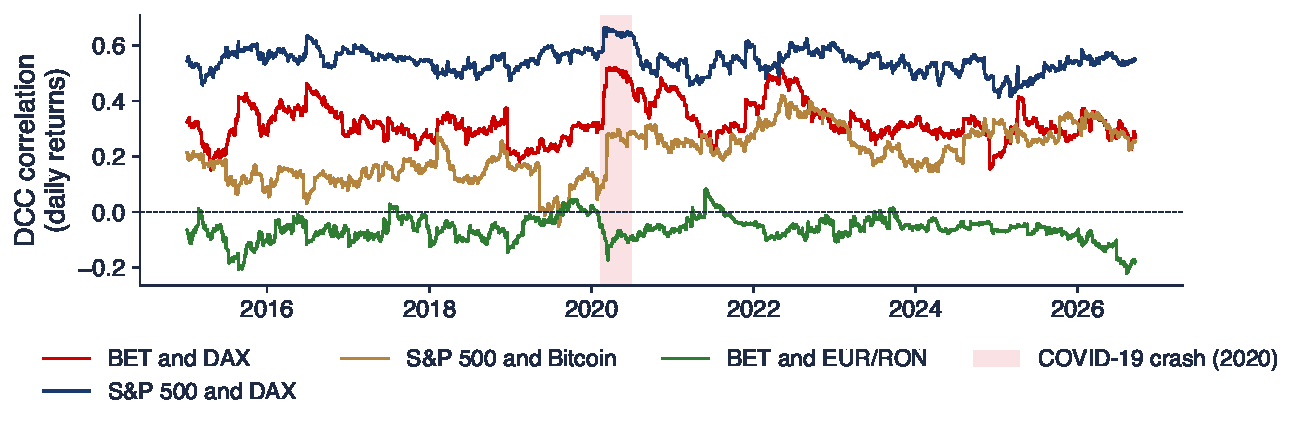
\includegraphics[width=0.97\textwidth,height=0.62\textheight,keepaspectratio]{tsa_ch14_panel_corr.pdf}
\end{center}
\vspace{-0.25cm}
\begin{itemize}
    \item One-step-ahead DCC correlations from the five-asset model; shaded: the COVID-19 crash, mid-February--June 2020
\end{itemize}
\quantlet{TSA\_ch14\_dcc\_panel}{\qlurl{TSA_ch14_dcc_panel}}
\end{frame}

\begin{frame}{Interpreting the four pairs}
\itemsize{\small}
\begin{itemize}
    \item S\&P 500 and DAX: the strongest link, mean 0.54; BET and DAX: mean 0.32, between 0.15 and 0.53 (April 2022)
    \item S\&P 500 and Bitcoin: from $-$0.05 to 0.42 (May 2022); mean 0.21
    \begin{itemize}
        \item the diversification benefit of Bitcoin shrank after 2020
    \end{itemize}
    \item BET and EUR/RON: close to zero (mean $-$0.06); a weaker leu tends to come with a weaker BET, a small negative link
    \item One $(a, b)$ for all pairs: pairs with different speeds are forced to the same rhythm, the price of DCC's parsimony
\end{itemize}
\end{frame}

\begin{frame}{Average correlations: calm against crisis}
\itemsize{\footnotesize}
\begin{center}
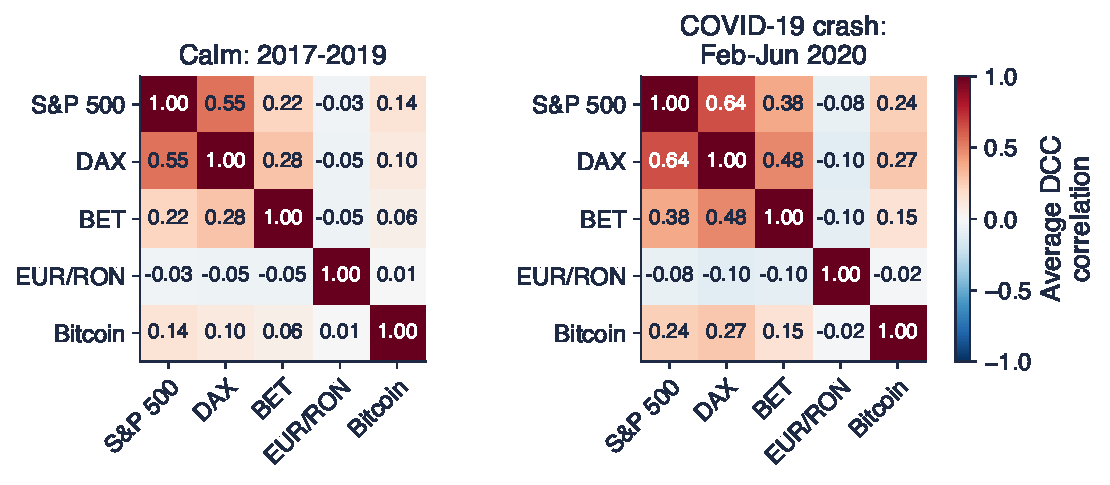
\includegraphics[width=0.97\textwidth,height=0.6\textheight,keepaspectratio]{tsa_ch14_panel_heatmap.pdf}
\end{center}
\vspace{-0.25cm}
\begin{itemize}
    \item Average one-step-ahead DCC correlation matrix: 2017--2019 and mid-February--June 2020 (89 common trading days)
\end{itemize}
\quantlet{TSA\_ch14\_dcc\_panel}{\qlurl{TSA_ch14_dcc_panel}}
\end{frame}

\begin{frame}{Interpreting the two matrices}
\itemsize{\small}
\begin{itemize}
    \item The average pairwise correlation rises from 0.12 to 0.19
    \begin{itemize}
        \item BET and DAX: 0.28 $\to$ 0.48; S\&P 500 and BET: 0.22 $\to$ 0.38; DAX and Bitcoin: 0.10 $\to$ 0.27
    \end{itemize}
    \item The largest rises are for the BET and for Bitcoin, which are weakly linked to the large markets in calm times: exactly the assets that were supposed to diversify
    \item EUR/RON stays near zero or slightly negative with all equity markets: the only diversifier in this set
\end{itemize}
\end{frame}

\begin{frame}{Recap: Five markets}
\itemsize{\small}
\begin{itemize}
    \item One DCC for 5 assets: 2 dynamics parameters for 10 correlations
    \item Correlations of the Romanian market with Europe and of Bitcoin with equities move a lot
    \item In the 2020 crash the weak links strengthened most: diversification weakens in crises
\end{itemize}
\end{frame}


%=============================================================================
\section{Portfolio VaR 1\% with DCC}
%=============================================================================

\begin{frame}{From $\mathbf{H}_t$ to the VaR of a portfolio}
\itemsize{\small}
\begin{itemize}
    \item Portfolio return $r_{p,t} = \mathbf{w}^\top\mathbf{r}_t$; conditional mean $\mu_p = \mathbf{w}^\top\boldsymbol{\mu}$ and volatility $\sigma_{p,t} = \sqrt{\mathbf{w}^\top\mathbf{H}_t\mathbf{w}}$
    \item \textbf{VaR 1\%}
    \begin{itemize}
        \item the loss exceeded with probability 1\%, $\mathrm{VaR}_{0.01,t} = -q_{0.01}(r_{p,t}) = -(\mu_p + q\,\sigma_{p,t})$
        \item Normal: $q = z_{0.01} = -2.326$
        \item \textbf{filtered historical simulation} (FHS): $q$ = the empirical 1\% quantile of the past standardised portfolio returns $(r_{p,t} - \mu_p)/\sigma_{p,t}$
    \end{itemize}
    \item Three choices of $\mathbf{H}_t$: DCC; CCC (GARCH volatilities with a constant correlation); \textbf{static} (one sample covariance matrix for all days)
\end{itemize}
\end{frame}

\begin{frame}{Worked example: VaR 1\% of two assets}
\itemsize{\small}
\begin{itemize}
    \item Today's forecasts: $\sigma_1 = 1.5\%$, $\sigma_2 = 1.2\%$ (daily), weights 50\% and 50\%, mean 0
    \item Calm, $\rho_t = 0.3$: $\sigma_p^2 = 0.25 \cdot 2.25 + 0.25 \cdot 1.44 + 2 \cdot 0.25 \cdot 0.3 \cdot 1.8$, so $\sigma_p = 1.092\%$ and VaR 1\% $= 2.326 \cdot 1.092 = 2.54\%$
    \item Crisis, $\rho_t = 0.9$ (the same volatilities): $\sigma_p = 1.316\%$ and VaR 1\% $= 3.06\%$
    \begin{itemize}
        \item the jump of the correlation alone adds a fifth to the VaR; in a real crisis the volatilities rise too
    \end{itemize}
    \item For a portfolio of 1 million lei: VaR 1\% of about 25.4 thousand lei in calm times and 30.6 thousand lei in the crisis case
\end{itemize}
\end{frame}

\begin{frame}{Backtesting a VaR (1/2): frequency}
\itemsize{\footnotesize}
\begin{itemize}
    \item A \textbf{violation} on day $t$
    \begin{itemize}
        \item $r_{p,t} < -\mathrm{VaR}_{0.01,t}$
        \item a correct VaR 1\% has violations on 1\% of the days, at random times
    \end{itemize}
    \item \textbf{Kupiec test} \refKupiec\ (frequency)
    \begin{itemize}
        \item $x$ violations in $n$ days, $\hat p = x/n$
        \item $LR_{uc} = -2\log\dfrac{(1-0.01)^{n-x}\,0.01^{x}}{(1-\hat p)^{n-x}\,\hat p^{x}} \sim \chi^2(1)$; reject at 5\% if $LR_{uc} > 3.84$
        \item $uc$: unconditional coverage; the ratio compares the likelihood of the violations under the rate 1\% with that under the observed rate $\hat p$
    \end{itemize}
\end{itemize}
\end{frame}

\begin{frame}{Backtesting a VaR (2/2): independence}
\itemsize{\footnotesize}
\begin{itemize}
    \item \textbf{Christoffersen test} \refChr\ (independence)
    \begin{itemize}
        \item is a violation more likely the day after a violation?
        \item compares $\pi_{11} = P(\text{violation} \mid \text{violation yesterday})$ with $\pi_{01} = P(\text{violation} \mid \text{no violation yesterday})$
    \end{itemize}
    \item The statistic
    \begin{itemize}
        \item $LR_{ind} = -2\log\dfrac{(1-\hat\pi)^{n_{00}+n_{10}}\,\hat\pi^{\,n_{01}+n_{11}}}{(1-\hat\pi_{01})^{n_{00}}\,\hat\pi_{01}^{\,n_{01}}\,(1-\hat\pi_{11})^{n_{10}}\,\hat\pi_{11}^{\,n_{11}}} \sim \chi^2(1)$
        \item $n_{ij}$: the number of days in state $j$ after a day in state $i$ (1: violation, 0: none); $\hat\pi_{01} = n_{01}/(n_{00}+n_{01})$, $\hat\pi_{11} = n_{11}/(n_{10}+n_{11})$
        \item $\hat\pi$: the overall violation rate; the numerator assumes $\pi_{01} = \pi_{11}$ (no clustering); a small $p$-value rejects independence
    \end{itemize}
    \item \textbf{Honest design}
    \begin{itemize}
        \item estimate all parameters on 2000--2014 (3\,712 days), then run the filters forward on 2015--2026 (2\,893 days) without re-estimating
    \end{itemize}
\end{itemize}
\end{frame}

\begin{frame}{VaR 1\% of an S\&P 500 and DAX portfolio, 2015--2026}
\itemsize{\footnotesize}
\begin{center}
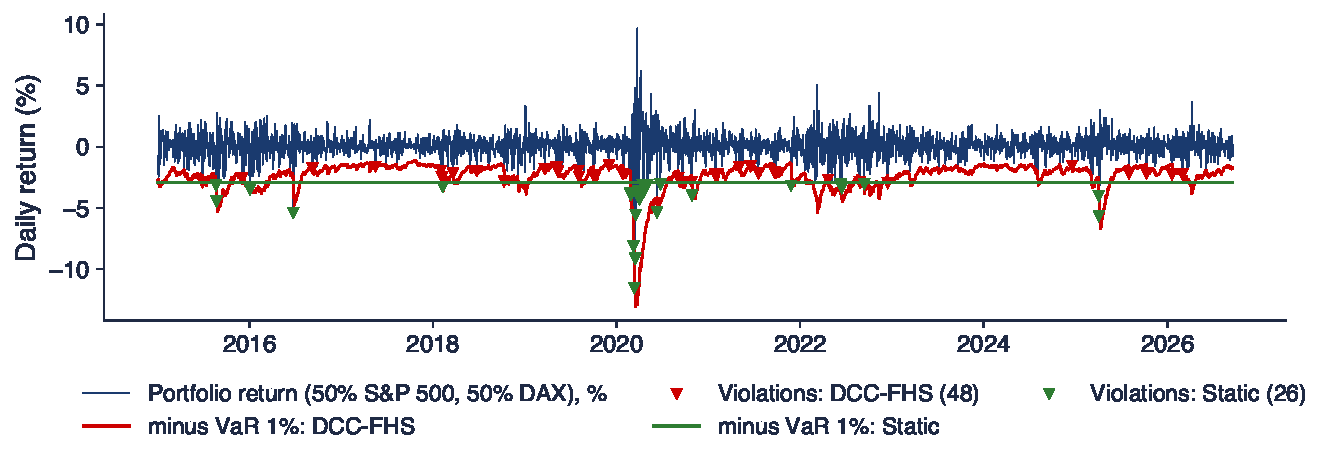
\includegraphics[width=0.97\textwidth,height=0.62\textheight,keepaspectratio]{tsa_ch14_var_backtest.pdf}
\end{center}
\vspace{-0.25cm}
\begin{itemize}
    \item Daily return of a 50/50 portfolio and minus VaR 1\% from DCC with filtered historical simulation and from a static covariance matrix; triangles: violations
\end{itemize}
\quantlet{TSA\_ch14\_portfolio\_var}{\qlurl{TSA_ch14_portfolio_var}}
\end{frame}

\begin{frame}{Interpreting the backtest}
\itemsize{\footnotesize}
\begin{center}
\footnotesize
\begin{tabular}{lrrrrrr}
\toprule
\textbf{Model} & Violations & Rate & $LR_{uc}$ & $p$ & $p$ indep. & Feb--Apr 2020 \\
\midrule
DCC, Normal & 65 & 2.25\% & 33.6 & $<$\,0.001 & 0.003 & 4 \\
DCC, FHS & 48 & 1.66\% & 10.6 & 0.001 & 0.008 & 4 \\
CCC, Normal & 57 & 1.97\% & 21.4 & $<$\,0.001 & 0.030 & 4 \\
Static, Normal & 26 & 0.90\% & 0.3 & 0.577 & 0.001 & 10 \\
\bottomrule
\end{tabular}
\end{center}
\begin{itemize}
    \item Expected: about 29 violations in 2\,893 days
    \item Dynamic models with Normal quantiles have too many violations: the residuals have fat tails (\tsachlink{https://danpele.github.io/Time-Series-Analysis/EN/Courses/chapter5_conditional_volatility_garch.pdf}{Chapter 5}); FHS ($q = -2.59$) brings the rate down to 1.66\%
    \item The static VaR passes the frequency test, but its violations cluster: 10 in February--April 2020 alone, and after a violation the next day is a violation with probability 11.5\%
    \item The static VaR is too high in calm years (2.95\% every day) and far too low in a crash; a dynamic VaR adapts in both directions
\end{itemize}
\end{frame}

\begin{frame}{Recap: Portfolio VaR}
\itemsize{\small}
\begin{itemize}
    \item $\sigma_{p,t} = \sqrt{\mathbf{w}^\top\mathbf{H}_t\mathbf{w}}$; VaR 1\% $= -(\mu_p + q\,\sigma_{p,t})$
    \item Backtest out of sample: Kupiec (frequency) and Christoffersen (independence)
    \item Dynamic covariances fix the clustering of violations; fat tails need a better quantile than the Normal
\end{itemize}
\end{frame}


%=============================================================================
\section{Dynamic hedge ratios}
%=============================================================================

\begin{frame}{The minimum-variance hedge ratio}
\itemsize{\footnotesize}
\begin{itemize}
    \item Hold one unit of asset $s$ (e.g. Romanian shares, the BET) and sell $h$ units of a hedging asset $f$ (e.g. a DAX futures contract)
    \begin{itemize}
        \item hedged return $r_{s,t} - h\,r_{f,t}$, with variance $\sigma_s^2 - 2h\,\sigma_{sf} + h^2\sigma_f^2$
        \item $\sigma_s^2$, $\sigma_f^2$: the variances of the two returns; $\sigma_{sf}$: their covariance
    \end{itemize}
    \item Setting the derivative in $h$ to zero: $h^* = \dfrac{\sigma_{sf}}{\sigma_f^2} = \rho\,\dfrac{\sigma_s}{\sigma_f}$ \refEd
    \begin{itemize}
        \item static $h^*$: the OLS slope of $r_s$ on $r_f$
        \item \textbf{dynamic}: $h_t^* = h_{sf,t}/h_{ff,t}$ from an MGARCH model \refKS; $h_{sf,t}$, $h_{ff,t}$: elements of $\mathbf{H}_t$
    \end{itemize}
    \item \textbf{Hedging effectiveness}
    \begin{itemize}
        \item $HE = 1 - \Var(r_s - h\,r_f)/\Var(r_s)$, the share of the variance removed
        \item with $h = h^*$ constant: $HE = \rho^2$; a hedge is only as good as the correlation
    \end{itemize}
\end{itemize}
\end{frame}

\begin{frame}{Worked example: a hedge ratio}
\itemsize{\small}
\begin{itemize}
    \item Given: $\sigma_s = 1.2\%$, $\sigma_f = 1.0\%$ (daily), $\rho = 0.8$
    \item Step 1: $\sigma_{sf} = \rho\,\sigma_s\sigma_f = 0.8 \cdot 1.2 \cdot 1.0 = 0.96$
    \item Step 2: $h^* = \sigma_{sf}/\sigma_f^2 = 0.96/1 = 0.96$: sell 0.96 units of $f$ per unit of $s$
    \item Step 3: $HE = \rho^2 = 0.64$; the hedged volatility is $\sigma_s\sqrt{1 - \rho^2} = 0.72\%$ instead of 1.2\%
    \item If tomorrow DCC forecasts $\rho_t = 0.5$ and $\sigma_{f,t} = 2\%$, the hedge ratio becomes $0.5 \cdot 1.2/2 = 0.3$: the position must be adjusted
\end{itemize}
\end{frame}

\begin{frame}{Hedging the BET with the DAX, 2015--2026}
\itemsize{\footnotesize}
\begin{center}
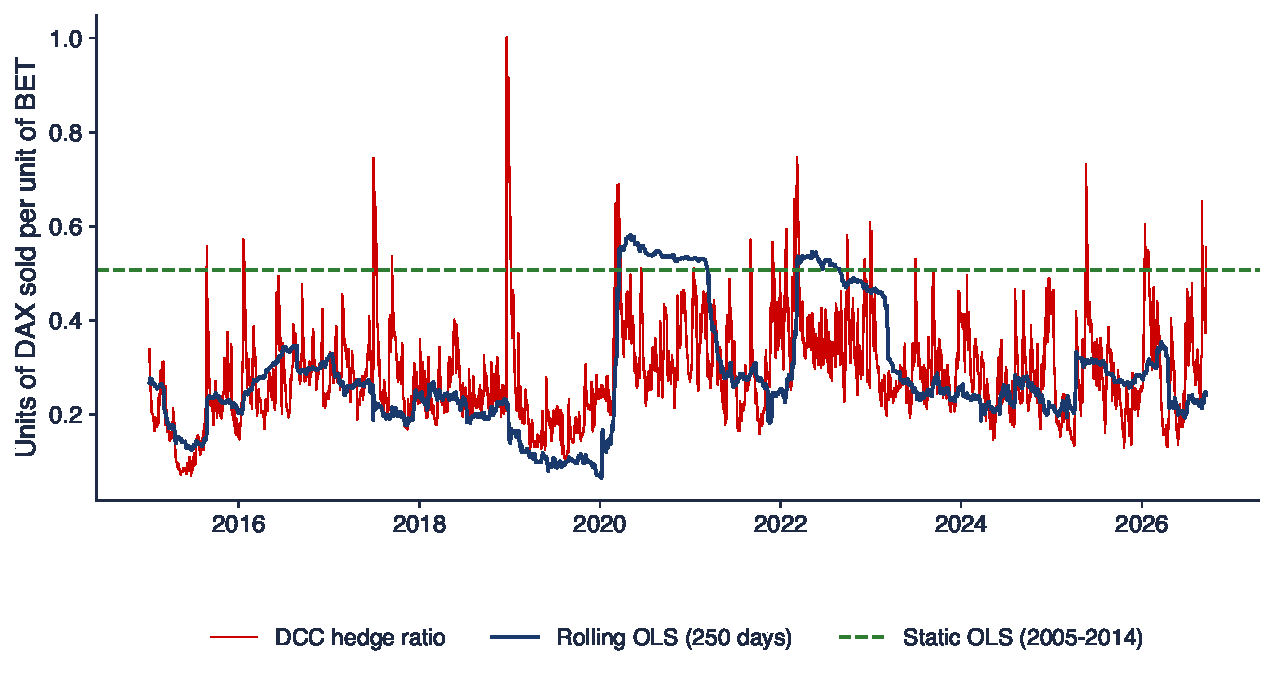
\includegraphics[width=0.97\textwidth,height=0.62\textheight,keepaspectratio]{tsa_ch14_hedge.pdf}
\end{center}
\vspace{-0.25cm}
\begin{itemize}
    \item Daily returns on common trading days since 2005; all parameters estimated on 2005--2014; DCC: $h_t = \hat\rho_t\hat\sigma_{BET,t}/\hat\sigma_{DAX,t}$; rolling OLS: the slope over the previous 250 days
\end{itemize}
\quantlet{TSA\_ch14\_hedging}{\qlurl{TSA_ch14_hedging}}
\end{frame}

\begin{frame}{Interpreting the hedge ratios}
\itemsize{\small}
\begin{itemize}
    \item The static ratio 0.51 reflects 2005--2014, which includes the 2008 crisis; after 2015 the DCC ratio averages 0.29, from 0.07 to 1.00 (20 December 2018)
    \item Hedging effectiveness out of sample (2\,893 days): static 13.6\%, rolling OLS 18.0\%, DCC 19.1\%
    \begin{itemize}
        \item the dynamic ratios remove more risk, and DCC does so without choosing a window
    \end{itemize}
    \item All effectiveness values are modest: the BET--DAX DCC correlation averages 0.32 since 2015, so $\rho^2$ is small
    \begin{itemize}
        \item a daily DCC ratio also implies daily trading costs, which are not counted here
    \end{itemize}
\end{itemize}
\end{frame}

\begin{frame}{Recap: Hedging}
\itemsize{\small}
\begin{itemize}
    \item $h_t^* = h_{sf,t}/h_{ff,t} = \rho_t\sigma_{s,t}/\sigma_{f,t}$; $HE = 1 - \Var(\text{hedged})/\Var(\text{unhedged})$
    \item BET with DAX: DCC 19.1\% against static 13.6\% out of sample
    \item Judge a hedge out of sample and after trading costs
\end{itemize}
\end{frame}


%=============================================================================
\section{Links with other chapters and limits}
%=============================================================================

\begin{frame}{Links with \tsachlinkt{https://danpele.github.io/Time-Series-Analysis/EN/Courses/chapter5_conditional_volatility_garch.pdf}{Chapters 5}, \tsachlinkt{https://danpele.github.io/Time-Series-Analysis/EN/Courses/chapter6_var_models_granger_causality.pdf}{6} and \tsachlinkt{https://danpele.github.io/Time-Series-Analysis/EN/Courses/chapter7_cointegration_vecm.pdf}{7}}
\itemsize{\small}
\begin{itemize}
    \item \textbf{\tsachlink{https://danpele.github.io/Time-Series-Analysis/EN/Courses/chapter5_conditional_volatility_garch.pdf}{Chapter 5}}
    \begin{itemize}
        \item every MGARCH model contains univariate GARCH models
        \item in DCC they are literally step 1
    \end{itemize}
    \item \textbf{\tsachlink{https://danpele.github.io/Time-Series-Analysis/EN/Courses/chapter6_var_models_granger_causality.pdf}{Chapter 6}}
    \begin{itemize}
        \item a VAR models spillovers in the \textbf{mean} (e.g.\ whether yesterday's DAX return helps to forecast today's BET return)
        \item BEKK with a full $\mathbf{A}$ models spillovers in the \textbf{variance}
        \item the two combine: a VAR for $\boldsymbol{\mu}_t$ and an MGARCH for $\mathbf{H}_t$; spillover indices from variance decompositions \refDY
    \end{itemize}
    \item \textbf{\tsachlink{https://danpele.github.io/Time-Series-Analysis/EN/Courses/chapter7_cointegration_vecm.pdf}{Chapter 7}}
    \begin{itemize}
        \item cointegration is a \textbf{long-run} link between price levels
        \item correlation is a \textbf{short-run} link between returns
        \item two prices can be highly correlated day by day and drift apart for ever, or cointegrated with low daily correlation
        \item a VECM can carry a DCC error term: equilibrium in the mean, dynamic correlation in the shocks
    \end{itemize}
\end{itemize}
\end{frame}

\begin{frame}{Limits and extensions}
\itemsize{\footnotesize}
\begin{columns}[T]
\begin{column}{0.34\textwidth}
\centering
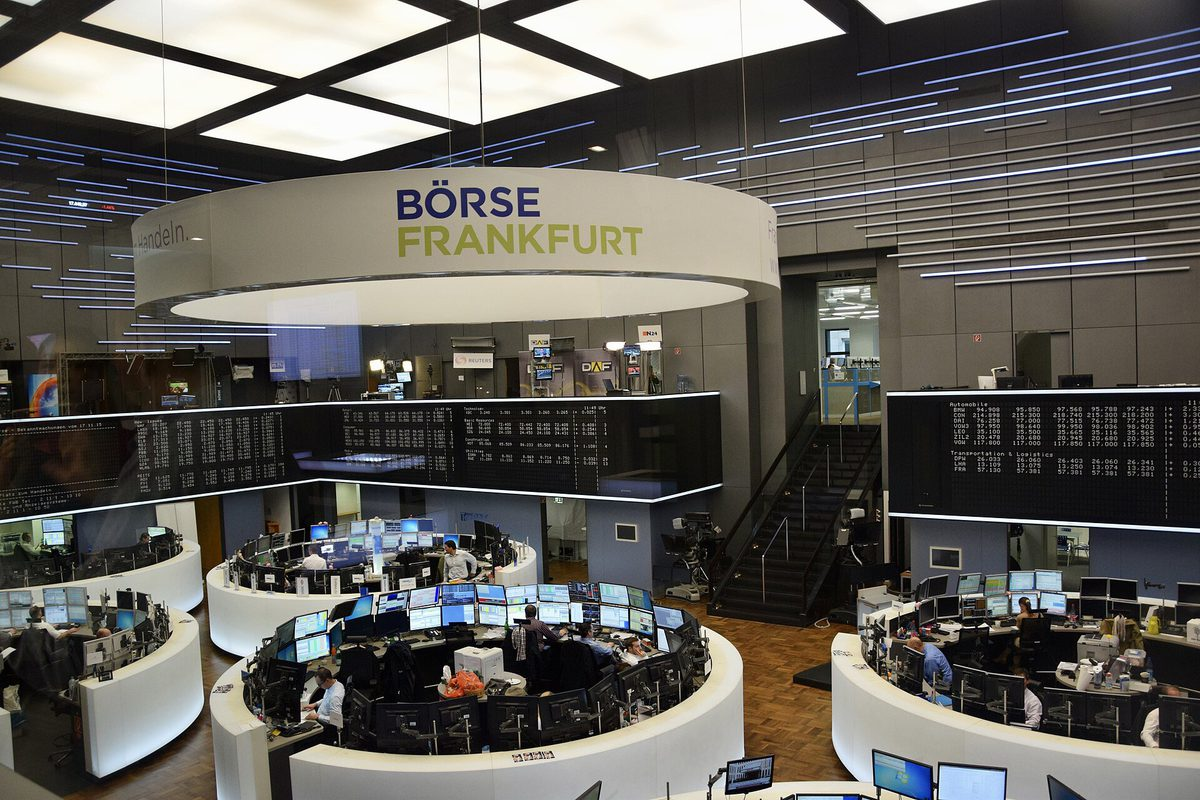
\includegraphics[height=0.3\textheight]{ch6_frankfurt_exchange_2015.jpg}\\[1mm]
\imgcap{Frankfurt Stock Exchange}
\imgcredit{https://commons.wikimedia.org/wiki/File:Frankfurt_Stock_Exchange_(Ank_Kumar)_01.jpg}{Photo: Ank Kumar (2015); CC BY-SA 4.0; Wikimedia Commons}
\end{column}
\begin{column}{0.64\textwidth}
\begin{itemize}
    \item One $(a, b)$ for all pairs; no spillovers between volatilities in DCC
    \item Normal QML underestimates the tails: use Student $t$ innovations or FHS for risk
    \item Asymmetry: correlations react more to joint falls (asymmetric DCC, \refCES)
    \item Hundreds of assets: factor models, composite likelihood and shrinkage of $\bar{\mathbf{Q}}$
    \item Correlation is linear dependence; for joint extremes see copulas and tail dependence \refLS
\end{itemize}
\end{column}
\end{columns}
\end{frame}


%=============================================================================
\section{Possible contribution of AI}
%=============================================================================

\begin{frame}{Possible contribution of AI}
\itemsize{\small}
\begin{itemize}
    \item \textbf{Code}
    \begin{itemize}
        \item a first draft of the DCC likelihood, of a BEKK filter, of a Kupiec test
    \end{itemize}
    \item \textbf{Explanation}
    \begin{itemize}
        \item a second explanation of $\mathbf{D}_t\mathbf{R}_t\mathbf{D}_t$, of correlation targeting, of the hedge-ratio formula
    \end{itemize}
    \item \textbf{Exploration}
    \begin{itemize}
        \item DCC for many pairs (CEE markets, sectors, currencies) and their behaviour in crises
    \end{itemize}
    \item Example prompt
    \begin{itemize}
        \item \aiprompt{Write Python code that fits a GARCH(1,1) to daily BET and DAX log returns on common trading days, estimates a DCC(1,1) model by two-step maximum likelihood with correlation targeting, plots the dynamic hedge ratio and compares its out-of-sample hedging effectiveness with static OLS.}
    \end{itemize}
\end{itemize}
\end{frame}

\begin{frame}{Checks you must run}
\itemsize{\small}
\begin{itemize}
    \item The library: \texttt{arch} has no DCC model; an AI answer that calls \texttt{arch\_model(..., vol='DCC')} has invented it
    \item The timing: $\mathbf{Q}_t$ must use $\mathbf{z}_{t-1}$, not $\mathbf{z}_t$; otherwise the VaR and the hedge use tomorrow's information
    \item The rescaling: $\rho_{ij,t} = q_{ij,t}/\sqrt{q_{ii,t}q_{jj,t}}$, and every $\mathbf{R}_t$ must have ones on the diagonal and $|\rho| < 1$
    \item The calendars: align prices on common trading days before computing returns; watch asynchronous closes
    \item The evaluation: estimate on one period and test on another; simulate a DCC with known $(a, b)$ and check that the code recovers it
    \item Every cited reference: it must exist; check the DOI
\end{itemize}
\end{frame}


%=============================================================================
\section{Summary}
%=============================================================================

\begin{frame}{Key takeaways}
\itemsize{\small}
\begin{itemize}
    \item Portfolio risk, hedging and contagion depend on time-varying covariances $\mathbf{H}_t$
    \item VEC is general but has too many parameters; BEKK is positive definite by construction and measures spillovers
    \item CCC and DCC split $\mathbf{H}_t = \mathbf{D}_t\mathbf{R}_t\mathbf{D}_t$ and are estimated in two steps; DCC needs only $(a, b)$ in step 2
    \item Real correlations move: integration, crises, new assets; constant correlation is rejected
    \item Applications: portfolio VaR 1\% with backtesting; dynamic hedge ratios judged out of sample
\end{itemize}
\end{frame}

\begin{frame}{Key formulas}
\itemsize{\small}
{\renewcommand{\arraystretch}{1.35}\begin{center}
\footnotesize
\begin{tabular}{ll}
\toprule
\textbf{Quantity} & \textbf{Formula} \\
\midrule
Correlation & $\rho_{ij,t} = h_{ij,t}/\sqrt{h_{ii,t}h_{jj,t}}$ \\
BEKK(1,1) & $\mathbf{H}_t = \mathbf{C}\mathbf{C}^\top + \mathbf{A}^\top\boldsymbol{\varepsilon}_{t-1}\boldsymbol{\varepsilon}_{t-1}^\top\mathbf{A} + \mathbf{B}^\top\mathbf{H}_{t-1}\mathbf{B}$ \\
CCC, DCC & $\mathbf{H}_t = \mathbf{D}_t\mathbf{R}_t\mathbf{D}_t$, \quad $\mathbf{D}_t = \mathrm{diag}(\sigma_{i,t})$ \\
DCC & $\mathbf{Q}_t = (1 - a - b)\bar{\mathbf{Q}} + a\,\mathbf{z}_{t-1}\mathbf{z}_{t-1}^\top + b\,\mathbf{Q}_{t-1}$, \quad $\rho_{ij,t} = q_{ij,t}/\sqrt{q_{ii,t}q_{jj,t}}$ \\
Half-life & $\ln 0.5/\ln(a + b)$ \\
Portfolio VaR 1\% & $-(\mathbf{w}^\top\boldsymbol{\mu} + q_{0.01}\sqrt{\mathbf{w}^\top\mathbf{H}_t\mathbf{w}})$ \\
Hedge ratio & $h_t^* = h_{sf,t}/h_{ff,t}$, \quad $HE = 1 - \Var(r_s - h r_f)/\Var(r_s)$ \\
\bottomrule
\end{tabular}
\end{center}
}
\end{frame}

\begin{frame}{Self-assessment (1/2)}
\itemsize{\footnotesize}
\begin{itemize}
    \item \textbf{Question}: how many parameters does a diagonal BEKK(1,1) have for $N = 3$?
    \begin{itemize}
        \item \textbf{Answer}: $N(N+1)/2 + 2N = 6 + 6 = 12$
    \end{itemize}
    \item \textbf{Question}: $h_{11} = 1$, $h_{22} = 4$, $h_{12} = 1.2$. What is the correlation, and is the matrix positive definite?
    \begin{itemize}
        \item \textbf{Answer}: $\rho = 1.2/\sqrt{4} = 0.6$; yes, $1 \cdot 4 - 1.44 > 0$
    \end{itemize}
    \item \textbf{Question}: DCC with $a = 0.02$, $b = 0.97$, $\bar q_{12} = 0.4$, $q_{11,t-1} = q_{22,t-1} = 1$, $q_{12,t-1} = 0.4$ and $z_{t-1} = (1, -1)$. What is $q_{12,t}$?
    \begin{itemize}
        \item \textbf{Answer}: $0.01 \cdot 0.4 + 0.02 \cdot (-1) + 0.97 \cdot 0.4 = 0.372$; opposite moves lower the correlation
    \end{itemize}
    \item \textbf{Question}: what is the half-life of correlation shocks when $a + b = 0.95$?
    \begin{itemize}
        \item \textbf{Answer}: $\ln 0.5/\ln 0.95 \approx 13.5$ days
    \end{itemize}
\end{itemize}
\end{frame}

\begin{frame}{Self-assessment (2/2)}
\itemsize{\footnotesize}
\begin{itemize}
    \item \textbf{Question}: $\sigma_s = 2\%$, $\sigma_f = 1\%$, $\rho = 0.5$. What are the hedge ratio and the hedging effectiveness?
    \begin{itemize}
        \item \textbf{Answer}: $h^* = 0.5 \cdot 2/1 = 1$; $HE = 0.25$
    \end{itemize}
    \item \textbf{Question}: a VaR 1\% has 26 violations in 2\,500 days, 10 of them in one month. Is it a good VaR?
    \begin{itemize}
        \item \textbf{Answer}: the frequency is fine (expected 25), but the violations cluster: it fails the independence test and does not adapt to crises
    \end{itemize}
    \item \textbf{Question}: why can the daily correlation of the S\&P 500 and the BET be lower than the weekly one?
    \begin{itemize}
        \item \textbf{Answer}: asynchronous trading: news from New York reaches Bucharest the next day, so daily returns of the same day do not match
    \end{itemize}
    \item \textbf{Question}: does a higher correlation in a crisis prove contagion?
    \begin{itemize}
        \item \textbf{Answer}: not by itself: higher volatility raises the sample correlation mechanically \refFR; compare correlations of standardised residuals
    \end{itemize}
    \item Next: \tsachlink{https://danpele.github.io/Time-Series-Analysis/EN/Courses/chapter15_review.pdf}{Chapter 15}, review and exam preparation; check yourself with the quiz of this chapter
\end{itemize}
\end{frame}


%=============================================================================
\section{References}
%=============================================================================

\begin{frame}{References (1/2)}
\itemsize{\scriptsize}
\begin{itemize}
    \item Aielli, G. P. (2013). Dynamic conditional correlation: On properties and estimation. \textit{Journal of Business \& Economic Statistics}, 31(3), 282--299. \href{https://doi.org/10.1080/07350015.2013.771027}{doi:10.1080/07350015.2013.771027}
    \item Bauwens, L., Laurent, S., \& Rombouts, J. V. K. (2006). Multivariate GARCH models: A survey. \textit{Journal of Applied Econometrics}, 21(1), 79--109. \href{https://doi.org/10.1002/jae.842}{doi:10.1002/jae.842}
    \item Bollerslev, T. (1986). Generalized autoregressive conditional heteroskedasticity. \textit{Journal of Econometrics}, 31(3), 307--327. \href{https://doi.org/10.1016/0304-4076(86)90063-1}{doi:10.1016/0304-4076(86)90063-1}
    \item Bollerslev, T. (1990). Modelling the coherence in short-run nominal exchange rates: A multivariate generalized ARCH model. \textit{The Review of Economics and Statistics}, 72(3), 498--505. \href{https://doi.org/10.2307/2109358}{doi:10.2307/2109358}
    \item Bollerslev, T., Engle, R. F., \& Wooldridge, J. M. (1988). A capital asset pricing model with time-varying covariances. \textit{Journal of Political Economy}, 96(1), 116--131. \href{https://doi.org/10.1086/261527}{doi:10.1086/261527}
    \item Cappiello, L., Engle, R. F., \& Sheppard, K. (2006). Asymmetric dynamics in the correlations of global equity and bond returns. \textit{Journal of Financial Econometrics}, 4(4), 537--572. \href{https://doi.org/10.1093/jjfinec/nbl005}{doi:10.1093/jjfinec/nbl005}
    \item Christoffersen, P. F. (1998). Evaluating interval forecasts. \textit{International Economic Review}, 39(4), 841--862. \href{https://doi.org/10.2307/2527341}{doi:10.2307/2527341}
    \item Diebold, F. X., \& Yilmaz, K. (2009). Measuring financial asset return and volatility spillovers, with application to global equity markets. \textit{The Economic Journal}, 119(534), 158--171. \href{https://doi.org/10.1111/j.1468-0297.2008.02208.x}{doi:10.1111/j.1468-0297.2008.02208.x}
    \item Ederington, L. H. (1979). The hedging performance of the new futures markets. \textit{The Journal of Finance}, 34(1), 157--170. \href{https://doi.org/10.1111/j.1540-6261.1979.tb02077.x}{doi:10.1111/j.1540-6261.1979.tb02077.x}
    \item Engle, R. F. (2002). Dynamic conditional correlation: A simple class of multivariate generalized autoregressive conditional heteroskedasticity models. \textit{Journal of Business \& Economic Statistics}, 20(3), 339--350. \href{https://doi.org/10.1198/073500102288618487}{doi:10.1198/073500102288618487}
\end{itemize}
\end{frame}

\begin{frame}{References (2/2)}
\itemsize{\scriptsize}
\begin{itemize}
    \item Engle, R. F., \& Kroner, K. F. (1995). Multivariate simultaneous generalized ARCH. \textit{Econometric Theory}, 11(1), 122--150. \href{https://doi.org/10.1017/S0266466600009063}{doi:10.1017/S0266466600009063}
    \item Forbes, K. J., \& Rigobon, R. (2002). No contagion, only interdependence: Measuring stock market comovements. \textit{The Journal of Finance}, 57(5), 2223--2261. \href{https://doi.org/10.1111/0022-1082.00494}{doi:10.1111/0022-1082.00494}
    \item Huang, C., \& Petukhina, A. (2022). \textit{Applied Time Series Analysis and Forecasting with Python}. Springer. \href{https://doi.org/10.1007/978-3-031-13584-2}{doi:10.1007/978-3-031-13584-2}
    \item Kroner, K. F., \& Sultan, J. (1993). Time-varying distributions and dynamic hedging with foreign currency futures. \textit{Journal of Financial and Quantitative Analysis}, 28(4), 535--551. \href{https://doi.org/10.2307/2331164}{doi:10.2307/2331164}
    \item Kupiec, P. H. (1995). Techniques for verifying the accuracy of risk measurement models. \textit{The Journal of Derivatives}, 3(2), 73--84. \href{https://doi.org/10.3905/jod.1995.407942}{doi:10.3905/jod.1995.407942}
    \item Longin, F., \& Solnik, B. (2001). Extreme correlation of international equity markets. \textit{The Journal of Finance}, 56(2), 649--676. \href{https://doi.org/10.1111/0022-1082.00340}{doi:10.1111/0022-1082.00340}
    \item Markowitz, H. (1952). Portfolio selection. \textit{The Journal of Finance}, 7(1), 77--91. \href{https://doi.org/10.1111/j.1540-6261.1952.tb01525.x}{doi:10.1111/j.1540-6261.1952.tb01525.x}
    \item Silvennoinen, A., \& Teräsvirta, T. (2009). Multivariate GARCH models. In T. G. Andersen et al.\ (Eds.), \textit{Handbook of Financial Time Series} (pp.~201--229). Springer. \href{https://doi.org/10.1007/978-3-540-71297-8_9}{doi:10.1007/978-3-540-71297-8\_9}
    \item Tse, Y. K. (2000). A test for constant correlations in a multivariate GARCH model. \textit{Journal of Econometrics}, 98(1), 107--127. \href{https://doi.org/10.1016/S0304-4076(99)00080-9}{doi:10.1016/S0304-4076(99)00080-9}
\end{itemize}
\end{frame}

\end{document}
